\documentclass[brudnopis]{xmgr}

\usepackage{listings}
\usepackage{color}
\usepackage{tabularx}
\usepackage[chapter]{minted}

\definecolor{dkgreen}{rgb}{0,0.6,0}
\definecolor{gray}{rgb}{0.5,0.5,0.5}
\definecolor{black}{rgb}{0.0,0.0,0.0}
\definecolor{mauve}{rgb}{0.58,0,0.82}

\newminted{javascript}{
  fontfamily=tt,
  linenos=true,
  numberblanklines=true,
  numbersep=12pt,
  numbersep=5pt,
  gobble=0,
  frame=leftline,
  framerule=0.4pt,
  framesep=2mm,
  funcnamehighlighting=true,
  tabsize=4,
  obeytabs=true,  
  mathescape=false
  samepage=true, 
  showspaces=false,
  showtabs =false,
  texcl=true,
}

\newminted{html}{
  fontfamily=tt,
  linenos=true,
  numberblanklines=true,
  numbersep=12pt,
  numbersep=5pt,
  gobble=0,
  frame=leftline,
  framerule=0.4pt,
  framesep=2mm,
  funcnamehighlighting=true,
  tabsize=4,
  obeytabs=true,  
  mathescape=false
  samepage=true, 
  showspaces=false,
  showtabs =false,
  texcl=true,
}

\newminted{java}{
  fontfamily=tt,
  linenos=true,
  numberblanklines=true,
  numbersep=12pt,
  numbersep=5pt,
  gobble=0,
  frame=leftline,
  framerule=0.4pt,
  framesep=2mm,
  funcnamehighlighting=true,
  tabsize=4,
  obeytabs=true,  
  mathescape=false
  samepage=true, 
  showspaces=false,
  showtabs =false,
  texcl=true,
}

% tak można zmienić domyślną rodzinę fontów Latin Modern 
%   na Minion + Myriad + Monaco:
%\defaultfontfeatures{Scale=MatchLowercase}
%\setmainfont[Mapping=tex-text]{Minion Pro:+onum}
%\setsansfont[Mapping=tex-text]{Myriad Pro}
%\setmonofont[Scale=0.75]{Monaco}

\wersja   {wersja wstępna [\ymdtoday]}

\author   {Patryk Jażdżewski}
\nralbumu {186507}
\email    {pjazdzewski@inf.ug.edu.pl}

\title    {Testowanie hybrydowych aplikacji mobilnych}
\date     {2014}
\miejsce  {Gdańsk}

\opiekun  {dr Wiesław Pawłowski}

\begin{document}

\begin{abstract}

  Poniższa praca zawiera opis biblioteki \textit{Ash} służącej do funkcjonalnego testowania
hybrydowych aplikacji mobilnych stworzonych przy użyciu Adobe PhoneGap lub
Apache Cordova. Ash pozwala na testowanie zachowania się aplikacji w~różnorodnych
realistycznych scenariuszach, które często są trudne do symulowania przez inne narzędzia. Tradycyjne podejścia nie pozwalają nam na testowanie aplikacji w~sytuacjach, gdy  użytkownik porusza się,
obraca ekran, traci dostęp do sieci i~tym~podobnych. Ash został stworzony z~myślą o~takich przypadkach. Dzięki wykorzystaniu hybrydowego charakteru aplikacji
możliwa jest emulacja zachowania, co wpływa na większy realizm testów, a~tym~samym na wiarygodność ich wyników. 
Biblioteka pozwala na budowanie złożonych scenariuszy z~prostych kroków, dzięki czemu struktura testów jest niezwykle elastyczna, a ich utrzymanie łatwe. 
Dodatkowo pozwala na wykorzystania asercji w~aplikacji nawet poza testami. 

\end{abstract}
\keywords{JavaScript, 
 Apache Cordova, 
 Adobe Phonegap,
testowanie,
hybrydowe aplikacje mobilne}

% tytuł i~spis treści
\maketitle

\introduction

Tematem pracy jest przedstawienie biblioteki Ash, problemów które stara się rozwiązać, możliwości jakie oferuje oraz zagadnień związanych z~jej~implementacją. Ten dokument  został stworzony z~myślą zarówno o~osobach myślących o~wykorzystaniu Ash-a w~ich projekcie, jak i~o~ludziach chcących zapoznać się ze sposobem działania biblioteki i~brać udział w~jej rozwoju.  

Pierwsze rozdziały wprowadzają czytelnika w~temat testowania aplikacji mobilnych oraz demonstrują jak skorzystać z~biblioteki do stworzenia prostych testów. Dalej następuje przegląd funkcjonalności oraz dyskusja na temat potencjalnych zastosowań. Kolejne rodziały opisują implementację najważniejszych części biblioteki oraz dają wgląd w~to,~jak można zintegrować Ash-a z~narzędziami do automatycznego budowania aplikacji.

\chapter{Podstawowe terminy oraz techniki}
\section{Hybrydowe aplikacje mobilne}
Mówiąc o~\textit{natywnej aplikacji mobilnej} mamy na myśli aplikację tworzoną z~myślą o~konkretnej platformie systemowej (Android, iOS, itp.) przy użyciu narzuconych przez jej twórcę narzędzi (Java, Objective-C, itd.).  \textit{Aplikacje mobile web} są to z~kolei aplikacje webowe zoptymalizowane po kątem urządzeń mobilnych.
Adobe PhoneGap oraz jej odpowiednik o~otwartym źródle Apache Cordova, to
dwie popularne biblioteki pozwalające na tworzenie \textit{hybrydowych aplikacji
mobilnych}, tj. aplikacji które łączą w~sobie zalety aplikacji natywnych oraz aplikacji
typu mobile web. Zasada działania tego typu programów jest w~założeniu prosta i~polega na wykorzystaniu komponentów, które dalej nazywać będziemy \textit{WebView}.
Komponenty te są dostępne na każdej nowoczesnej platformie i~pozwalają na
wyświetalnie stron internetowych z~wnętrza natywnych aplikacji mobilnych. 
W momencie startu aplikacja hybrydowa tworzy WebView oraz ładuje do niego zasoby z~określonego adresu (lokalnego lub zdalnego). Najczęściej zasobem jest aplikacja stworzona przy użyciu technologii webowych.     

% tabelki w~LaTeX-u też da się robić, chociaż najczytelniej to może nie wygląda
% więcej na temt tabelek można poczytac np. na http://en.wikibooks.org/wiki/LaTeX/Tables

\begin{center}
    \begin{tabularx}{\textwidth}{ | X | X | X | X |}
    \hline & Aplikacje naty\-wne&Aplikacje hybrydowe&Aplikacje mobile web\\ 
    \hline Narzędzia&Zależne od platformy	&Narzędzia webowe&Narzędzia webowe\\
    \hline Instalacja&Wymagana&Wymagana&Nie wymagana\\ 
    \hline Wydajność&Bardzo dobra&Ograniczona przez WebView&Ograniczona przez używaną przeglądarkę\\ 
   \hline Możliwość monetyzacji&Pobranie, reklamy, subskrybcje&Pobranie, reklamy, subskrybcje&Subskrybcje, reklamy\\ 
  \hline Dostęp do urządzenia&Tak, pełen&Najważniejsze funkcjonalności& Ograniczony\\ 
  \hline
  \end{tabularx}
\end{center}

Takie podejście ma wiele zalet. Dzięki temu, że do tworzenia aplikacji hybrydowych wykorzystywane są powszechnie znane technologie internetowe, koszt ich tworzenia i~czas dostarczenia
gotowego rozwiązania na rynek są znacznie zredukowane. Aplikacje tego typu są też
z~założenia wieloplatformowe. Używając PhoneGap z~tego samego kodu źródłowego
możemy stworzyć aplikacje na platformę Android, iOS, Blackberry, WebOS,
Windows Phone, Symbian i~Bada. Dodatkowo popularność narzędzi internetowych
ułatwia znalezienie właściwych programistów.

\section{Wady podejścia hybrydowego}
Największymi wadami podejścia hybrydowego są słabsza wydajność, błędy
pojawiające się tylko na określonych urządzeniach oraz potencjalnie odmienne oczekiwania użytkowników różnych platform. 

Użytkownik instalując aplikację hybrydową w~taki sam sposób co 
natywną spodziewa się, że będzie ona działać niczym natywna. Tymczasem
dodatkowy narzut hybrydy, często w~połączeniu z~niedopracowaną i~nie
zoptymalizowaną aplikacją, prowadzi do mało responsywnego interfejsu
użytkownika i~w~konskewencji do frustracji użytkownika. Częstym problemem przy
tworzeniu aplikacji mobilnych są błędy, które są specyficzne tylko dla pewnych modeli urządzeń. Przy podejściu hybrydowym problem jest o~tyle bardziej widoczny, że
najczęściej tworzymy rozwiązanie które ma być przenośne nie tylko pomiędzy urządzeniami w~ramach jednej platformy, ale także między platformami. Z~oczywistych względów zwiększa to gamę urządzeń, które trzeba uzwględnić. Trzecim problemem hybryd jest kwestia
tworzenia interfejsu użytkownika tak, aby był intuicyjny i~wygodny dla użytkownika. Dostawcy systemów operacyjnych dla urządzeń
mobilnych publikują zalecenia, co do tego jak powinien wyglądać i~zachowywać się interfejs aplikacji
działającej pod danym systemem. Zalecenia te są specyficzne dla platformy i~często
wzajemnie się wykluczają. Przygotowanie jednej szaty graficznej i~jednego interfejsu
może zostać źle odebrane przez użytkowników spodziewających się wyglądu
dostosowanego do platformy. Niestety stworzenie kilku wersji interfejsu jest dużo
bardziej pracochłonne i~skomplikowane. Niweczy także podstawową zaletę aplikacji
hybrydowych – przenośność. 
Są to poważne niedostatki, ale braki te można zniwelować z~pomocą skutecznych narzędzi.

\section{Propozycja rozwiązania problemów}
Ash ma za zadanie pomóc rozwiązywać problemy z~wydajnością aplikacji oraz z~błędami zależnymi od konfiguracji sprzętowych. Aby
zapewnić wysoką sprawność działania aplikacji konieczny jest rygor przy tworzeniu
oprogramowania oraz możliwość testowania jej w~sytuacjach, które pozwalają
uwydatnić problemy z~wydajnością. Dzięki \textit{funkcyjnemu} podejściu do testowania
oprogramowania Ash pozwala zbierać informacje o~responsywności interfejsu
oraz realistycznie symulować scenariusze dużego obciążenia. Programista
korzystający z~Ash-a ma możliwość zdefiniowania w~scenariuszach maksymalnego
czasu trwania testu. Jeśli test nie zakończy się w~założonym czasie jest on oznaczany jako niepowodzenie. Niska responsywność interfejsu traktowana jest na równi z~błędami
logiki czy prezentacji. Wymusza to na twórcy dbanie o~szybkość reakcji aplikacji.
Ash oferuje także możliwość chwilowego wyłączenia lub opóźnienia dostępu do
sieci. Sytuacje w~których dostępność internetu jest ograniczona są dość częste,
jednak niewiele programów jest pisanych biorąc to pod uwagę, a~jeszcze mniej 
testowana pod tym kątem. Bardzo często problemy z~dotępem do sieci objawiają się kiepską
wydajnością interfejsu lub długimi przestojami na ekranach ładowania. Ash pozwala
twórcom świadomie zmierzyć się z~tym problemem. Biblioteka wyposażona jest także w~mechanizmy pozwalajace na łatwe uruchomienie aplikacji na wielu urządzeniach, fizycznych i~wirtualnych naraz -- nawet w~zdalnych lokalizacjach. Sprawia to, że
użytkownicy mają możliwość masowego uruchamiania testów na wszystkich
dostępnych im urządzeniach oraz są bardziej skłonni skorzystać z~testów w~czasie
swojej pracy. Zdalne uruchamianie testów daje możliwość stworzenia
rozproszonej bazy urządzeń, co pozwoli na testowanie także mniej typowych
konfiguracji.

\section{Dlaczego Apache Cordova}
Jako bazę do implementacji wybrałem Apache Cordova. Jest to
wersja PhoneGap, którą korporacja Adobe (właściel praw do PhoneGap) udostępniła
fundacji Apache. Od tego momentu ten wariant technologii udostępniany jest
na zasadzie otwartego źródła. Pomimo tego, oba projekty są niemal identyczne, a~jedyna faktyczna różnica między nimi jest natury prawnej. Głównym powodem
wyboru tej technologii jest spory udziała w~rynku hybrydowych aplikacji mobilnych,
dynamizm rozwoju oraz liczna społeczność użytkowników. Nie bez znaczenia jest także swobodny dostęp do źródła biblioteki.

Więcej informacji na temat historii projektu można znaleźć w~książce Johna Wargo \cite{Wargo}. 

\section{Test Driven Development}

\textit{Test Driven Development} (w skrócie TDD) jest to metodologia wytwarzania oprogramowania opierająca się na krótkich cyklach programistycznych, o~których często mówimy \textit{red--green--refactor}. Na taki cykl składają się następujące fazy.
\begin{itemize}
  \item \textit{Red} -- Programista pisze testy automatyczne, pokrywające funkcjonalność, która została wyspecyfikowana, ale nie została jeszcze zaimplementowana. Na tym etapie testy oczywiście nie przechodzą.
  \item \textit{Green} -- Następnie programista implementuje brakujące funkcjonalności, aż wszystkie testy napisane w~poprzednim kroku staną się ,,zielone'', czyli uruchamiają się i~kończą bez błędów.
  \item \textit{Refactor} -- Na tym etapie testowana aplikacja jest udoskonalana. Dzięki testom nie ma obawy, że nowe funcjonalności czy poprawki doprowadzą do regresji, do błędów w~działaniu elementów, które wcześniej funkcjonowały poprawnie. Wszelkie takie przypadki powinny zostać wykryte przez testy automatyczne. Po zakończeniu implementacji tworzone są dodatkowe pokrywające poszerzony zakres funkcjonalności.
\end{itemize}

Dzięki zastosowaniu krótkich cykli oraz automatycznych testów, metodologia TDD pozwala na tworzenie oprogramowania, które ma przemyślaną architekturę oraz unika problemów związanych z~regresją. Tworząc kod  programu programista musi dopilnować, aby jego kod był testowalny, co prowadzi do poprawienia jakości tworzonego oprogramowania. Testy automatyczne, które powstają podczas cyklu zwiększają prawdopodobieństwo, że w~przypadku, gdy kod aplikacji zmieni się, potencjalne błędy zostaną od razu wychwycone. 

Test Driven Developement jako metodologia jest powiązana z~\textit{Extreme Programming} oraz z~koncepcją \textit{Tests First}, która zakłada, że zestawy testów automatycznych powinny być tworzone jeszcze przed napisaniem testowanej aplikacji.

Metodologia TDD została spopularyzowana przez Kenta Becka \cite{Beck}.
\footnote{
Więcej informacji na teamt TDD można znaleźć na stronach:

\url{http://www.agiledata.org/essays/tdd.html}

\url{http://msdn.microsoft.com/en-us/library/aa730844(v=vs.80).aspx}
}

\section{Hierarchia testów}

Wyróżniamy wiele rodzajów testów. Poniżej krótko zostały scharakteryzowane niektóre z~nich.
\begin{itemize}
  \item Jednostkowe -- Testy obejmujące poszczególne funkcje na najniższym poziomie. Ich wykonywanie musi być możliwie jak najszybsze. Nie powinny korzystać z~zewnętrznych zasobów.
  \item Integracyjne -- Ten rodzaj testów pokrywa wiele komponentów aplikacji naraz i~testuje nie tylko, czy każdy z~poszczególnych modułów działa poprawnie w~izolacji, ale także czy komunikacja między nimi jest poprawna.
  \item Funkcyjne -- Testy tego typu sprawdzają, czy interfejs aplikacji jest poprawny oraz czy interakcja z~użytkownikiem działa poprawnie. U~podstaw ich działania leży symulowanie zachowania programu jak gdyby operowali na nim ludzie. 
  \item A/B -- Tak zwane testy A/B polegają na testowaniu oprogramowania pod kątem wygody i~praktyczności interfejsu.
  \item Wydajnościowe -- Jak sama nazwa wskazuje służą one do sprawdzenia wydajności aplikacji.
\end{itemize}

W~przypadku poprawnie zarządzanego projektu trzy pierwsze rodzaje tworzą hierarchię zwaną \textit{piramidą testowania}. Dwa pozostałe z~wymienionych przeze mnie rodzajów pełnią funkcję uzupełniającą. 
\footnote{
Informacje na temat piramidy testów oraz ich rozkładu w~aplikacjach można znaleźć na stronach:

\url{http://martinfowler.com/bliki/TestPyramid.html}

\url{http://www.duncannisbet.co.uk/test-automation-basics-levels-pyramids-quadrants}
}

\begin{figure}[h]
    \centering
    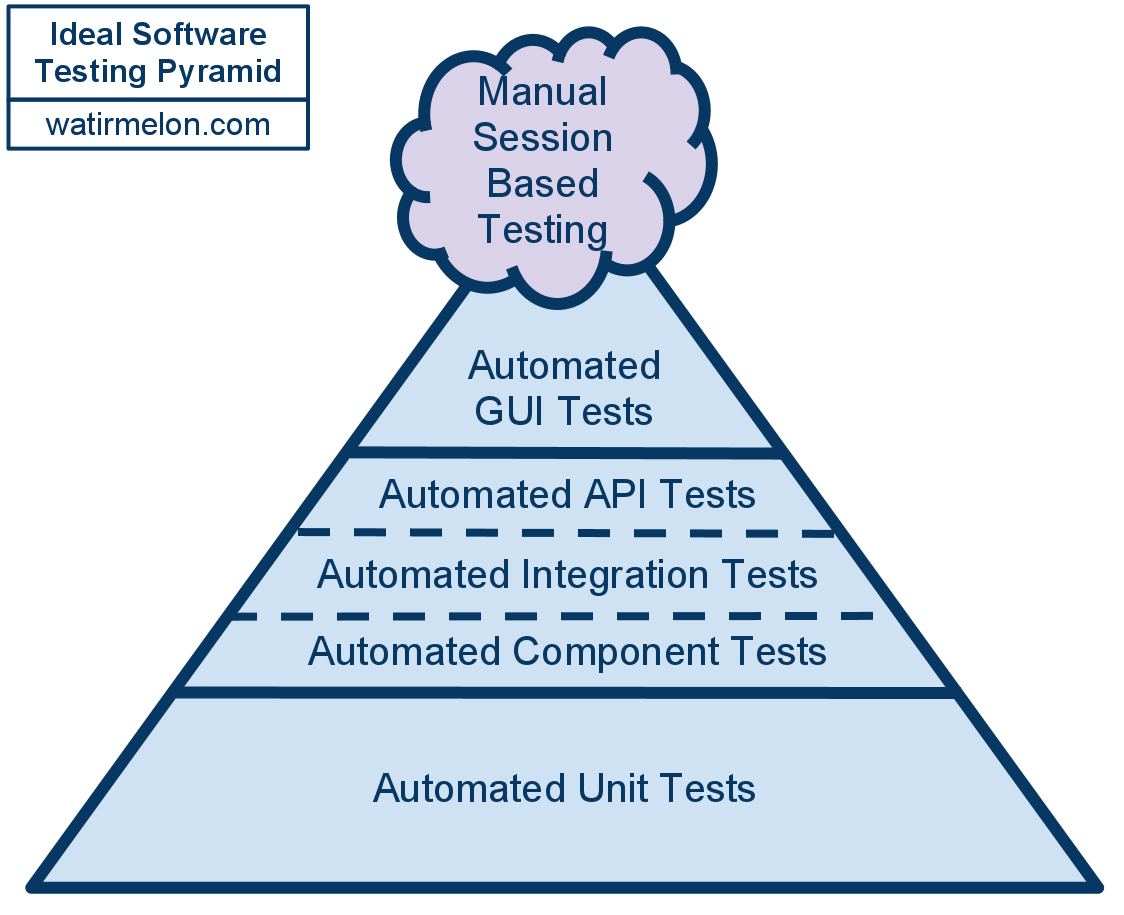
\includegraphics[scale=0.25]{idealautomatedtestingpyramid.png}
    \caption{Piramida testów}
    \label{fig:pyramis}
\end{figure}

Biblioteka Ash została stworzona z~myślą o~testowaniu funkcyjnym.

\chapter{Sposób użycia}
\section{Pierwsze kroki}

Aby dołączyć Ash-a do swojego projektu należy wydać następujące polecenie\footnote{Jeśli nie masz zainstalowanego Cordova CLI spójrz tutaj \url{https://github.com/apache/cordova-cli} } w~folderze z~projektem:
\begin{quote}
   \texttt{cordova plugins add https://github.com/pjazdzewski1990/Ash}
\end{quote}

Wtyczka zostanie zainstalowana, a~do~globalnej przestrzeni nazw dodany zostanie obiekt Ash, który udostępnia wszystkie metody biblioteki.

Punktem startowym Ash-a jest metoda \texttt{loadTests}. Przyjmuje ona tablicę ścieżek do plików zawierająych kod z~testami. Po wywołaniu dynamicznie dodaje wskazane pliki do dokumentu w~ramach którego została wywołana. Pliki z~testami należy napisać samodzielnie pamiętając, żeby były one zamknięte w~ramach \textit{self--invoking--function}. Takie podejście służy temu, aby umożliwić użytkownikowi łatwe dodanie i~usunięcie testów z~aplikacji oraz aby testy niepotrzebnie nie zaśmiecały produkcyjnej wersji aplikacji.

Projekt demonstrujący użycie Ash-a oraz jego możliwości jest dostępny pod adresem

\url{https://github.com/pjazdzewski1990/AshDemo}

\section{Hello World}

Na porzeby wprowadzenia do testowania przy użyciu Ash-a powstała aplikacja AshHello, która jest dostępna pod adresem 

\url{https://github.com/pjazdzewski1990/AshHello}

Aby pobrać projekt wydaj polecenie

\begin{quote}
   \texttt{git clone git@github.com:pjazdzewski1990/AshHello.git}
\end{quote}

Aplikacja AshHello oferuje bardzo prostą funkcjonalność. Jej zasadniczym celem jest zaznajomienie użytkownika z~testowaniem przy użyciu biblioteki Ash. Interfejs użytkownika w~AshHello jest zorganizowany na zasadzie tzw. {\it Working Square}. Working Square jest to wzorzec tworzenia interfejsu, bardzo popularny na urządzeniach mobilnych. Polega on~na stworzeniu kwadratowego obszaru roboczego który zawiera główną treść aplikacji oraz obszaru pomocniczego na którym znajdować się mogą np. elementy związane z~nawigacją. W~zależności od orientacji ekranu, która dyktuje nam rozmiar i~kształt powierzchni do zagospodarowania, obszar pomocniczy może znajdować się 

\begin{itemize}
  \item poniżej obszaru głównego -- gdy urządzenia jest w~orientacji pionowej, tzn. wysokość ekranu jest większa niż jego szerokość,

\begin{figure}[h]
    \centering
    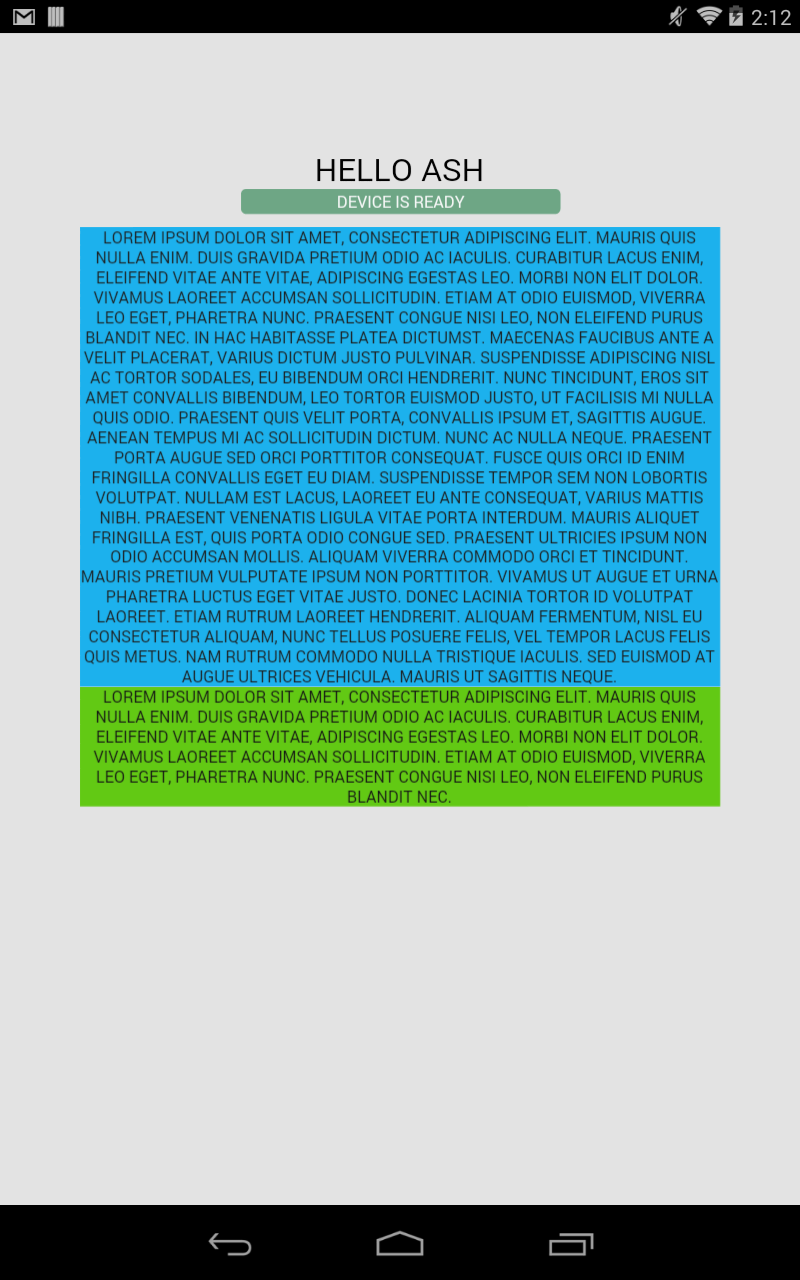
\includegraphics[scale=0.25]{hello1.png}
    \caption{AshHello w~orientacji pionowej}
    \label{fig:AshHello1}
\end{figure}

  \item obok obszaru głównego -- gdy urządzenie jest w~orientacji poziomej, czyli szerokość dostępnego ekranu jest większa niż jego wysokość.

\begin{figure}[h]
    \centering
    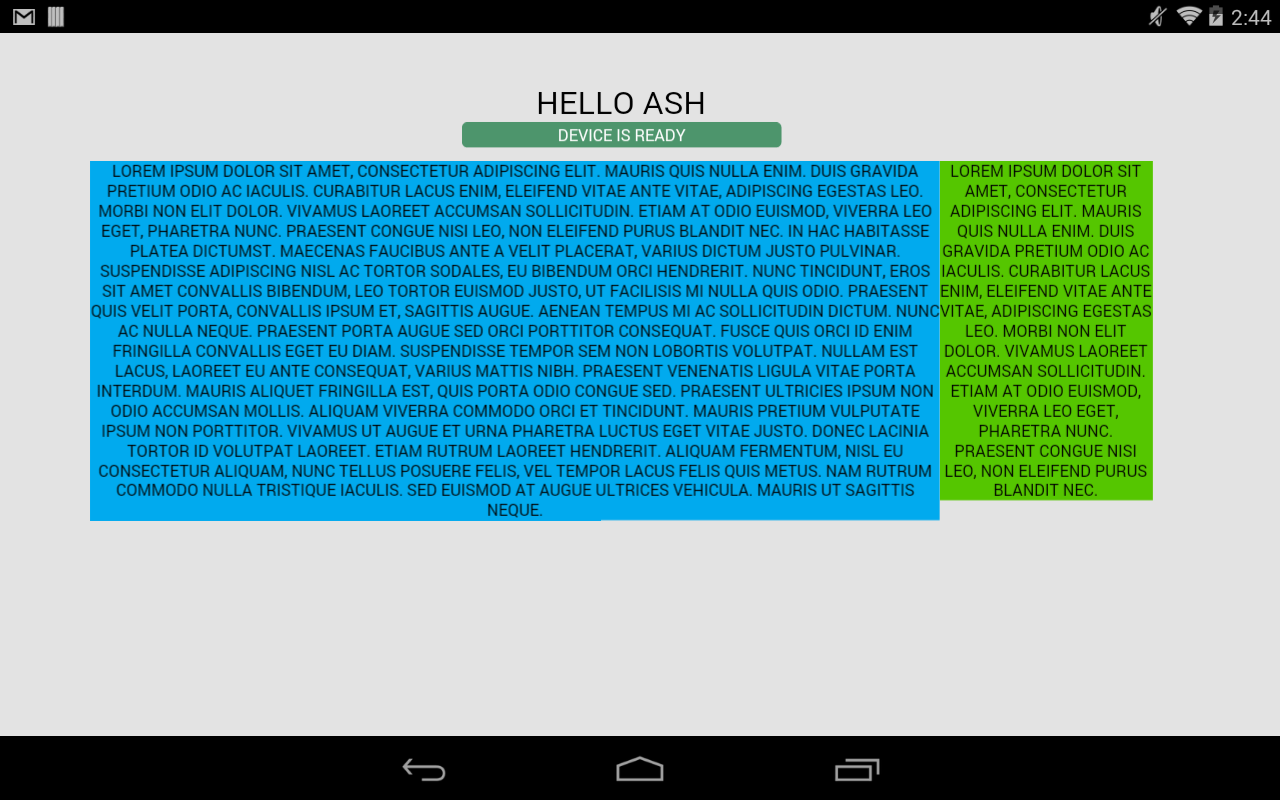
\includegraphics[scale=0.25]{hello2.png}
    \caption{AshHello w~orientacji poziomej}
    \label{fig:AshHello2}
\end{figure}
\end{itemize}

Poniższa intrukcja krok~po~kroku wyjaśni, jak dodać testy Ash--a do projektu AshHello. Dla większej przejrzystości demonstracji testy będą korzystać z~popularnej biblioteki \textit{jQuery}\footnote{Dostępna pod \url{http://jquery.com/}}, chociaż jej dołączenie nie jest wymagane, gdy pracujemy z~Ash.  

\begin{enumerate}
  \item Dodajemy Ash-a do projektu korzystając z~Cordova CLI.

Wtyczkę instalujemy poleceniem 
\begin{quote}
   \texttt{cordova plugins add https://github.com/pjazdzewski1990/Ash}
\end{quote}
i~jeśli wszystko przebiegło poprawnie, to zmienna \texttt{window.Ash} powinna zawierać obiekt udostępniający funkcjonalność biblioteki.  

 \item Tworzymy plik z~testami

W folderze projektu tworzymy katalog 
\begin{quote}
  \texttt{www/test/}
\end{quote} 
a w~nim plik 
\begin{quote}
  \texttt{myTest.js}
\end{quote} 
W przed chwilą stworzonym pliku definiujemy samowywołującą się funkcję, która będzie zawierać nasze testy. Możemy  to zrobić na przykład w~następujący sposób:

 \begin{javascriptcode}
  (function(){
	console.log("MyTest started!");
	//  tu znajdzie się kod testujący 
  })();
\end{javascriptcode}

Powyższa funkcja zostanie wywołana zaraz po jej wczytaniu. Nasze testy nie będą zbyt skomplikowane, więc pozwolimy sobie na umieszczenia całej logiki bezpośrednio w~tej funkcji. Jednak w~przypadku bardziej rozbudowanych testów warto pokusić się o~zgromadzenie kodu w~obiektach.

Mamy zamiar sprawdzić, czy Working Square działa poprawnie w~obu ustawieniach ekranu, więc musimy skorzystać z~\textit{kontekstów}. Kontekstami będziemy nazywać funkcje, które gwarantują nam, że w~obrębie ich działania zachodzić będą określone warunki. Przykładem kontekstów są na przykład

\begin{quote}
   \texttt{Ash.orientationHorizontal()}
\end{quote}

oraz 

\begin{quote}
   \texttt{Ash.orientationVertical()}
\end{quote}

które pozwalają na odwrócenie ekranu. W~obrębie funkcji przekazanych jako argumenty do tych kontekstów, możemy być pewni, że ekran znajdzie się w~takim, a~nie innym położeniu. Korzystamy z~nich w~następujący sposób

 \begin{javascriptcode}
  //myTest.js

  Ash.orientationHorizontal().then(function(msg){
     //ten kod będzie wywołany, gdy ekran 
     // znajdzie się w orientacji poziomej
      var worksquare = $('.worksquare');
      var sidebar = $('.sidebar');

      Ash.assert(worksquare);
      Ash.assert(sidebar);

      Ash.equal(worksquare.getBoundingClientRect().top,
           sidebar.getBoundingClientRect().top);
     Ash.assert(worksquare.getBoundingClientRect().left <
           sidebar.getBoundingClientRect().left);

      Ash.endTest();
    });  
\end{javascriptcode}

Powyższy test sprawdza trzy rzeczy. Po pierwsze znajduje elementy interfejsu, które chcemy zbadać. Przy użyciu 

\begin{quote}
  \texttt{Ash.assert( ... )} 
\end{quote}

upewnia się, że istnieją. A następnie porównuje ich pozycje upewniając się, że elementy są ułożone obok siebie i~we właściwej kolejności. Ostanią operacją jest \texttt{Ash.endTest()} co oznacza zakończenie testu sukcesem.

Póki co nasz test obejmuje tylko część funkcjonalności. Musimy też zadbać o~orientację pionową oraz~o~to, czy przejście nie ,,psuje'' interfejsu. Aby to zbadać możemy dodać dalszą część testu. Na przykład w~ten sposób

 \begin{javascriptcode}
  //myTest.js

  Ash.orientationHorizontal().then(function(msg){
       //kod zporzedniego punktu

      //to jeszcze nie koniec testu, 
      //  więc musimy ująć w komentarz lub usunąć endTest()
      //Ash.endTest();
  }).then(
      Ash.orientationVertical //a teraz odwróć ekran pionowo
    ).then(function(msg){
      var worksquare = $('.worksquare');
      Ash.assert(worksquare);
      
      var sidebar = $('.sidebar');
      Ash.assert(sidebar);

      Ash.assert(worksquare.getBoundingClientRect().top <
sidebar.getBoundingClientRect().top);
      Ash.equal(worksquare.getBoundingClientRect().left,
sidebar.getBoundingClientRect().left);        

      //jesli aplikacja dotarła tutaj,
      //  to zaliczmy ten przypadek testowy
      Ash.endTest();
    });
\end{javascriptcode}

Powyższy kod nie jest bardziej skomplikowany od poprzedniego. Jedyną nowością jest zastosowanie wielu bloków 

\begin{quote}
  \texttt{then(function(){ ... })}
\end{quote}

które są wykonywane jeden po drugim w~kolejności podania i~pozwalają nam łączyć mniejsze funkcje testujace w~bardziej złożone bloki.

 \item Dodajemy wywołanie kodu testującego do aplikacji

Teraz kiedy mamy już kod testów czas dodać go do aplikacji. W~przypadku AshHello dobrym na to miejscem będzie \texttt{index.js} i~metoda \mbox{\texttt{onDeviceReady()}}. Metoda ta jest wywołana, gdy zajdzie już zdarzenie \texttt{deviceready} więc jesteśmy w~stanie skorzystać ze~wszystkich dobrodziejstw Apache Cordova.

 \begin{javascriptcode}
  //index.js
  
  var app = {
	...
    onDeviceReady: function() {
        console.log('Received onDeviceReady Event');
        app.setupUI();
        app.runAshTests();
    },
    runAshTests: function() {
        window.onerror = function(errorMsg, url, lineNumber) {
            alert("Error "+url+":"+lineNumber+"\n" + errorMsg);
        };
        Ash.loadTests(["test/myTest.js"]);
    },
	...
  };

\end{javascriptcode}

Metoda \texttt{runAshTests()} robi dwie rzeczy. Dodaje wywołanie zwrotne dla zdarzenia onerror oraz ładuje testy. W~tym uproszczonym scenariuszu chcemy, żeby wszystkie znalezione błędy objawiały się wyskującym okienkiem z~opisem problemu. Następnie korzystając z~dotarczonej przez Ash-a metody \texttt{loadTests()} ładujemy\texttt{ myTests.js}, jeśli przypomnimy sobie jak skonstruowany jest ten plik jasne stanie się, że od razu po wczytaniu zostanie on uruchomiony. 

\end{enumerate}

Tak niewiele potrzeba, żeby stworzyć i~uruchomić pierwszy prosty test Ash. W~razie problemów z~uruchomieniem działający kod testowy znajduje~się w~gałęzi ,,with--tests''.

\section{Podejście do tworzenia testów}

Ash oferuje dużą swobodę jeśli chodzi o~tworzenie zestawów testów przez użytkownika, jednocześnie sugeruje dobre praktyki, które pozwalają w~pełni wykorzystać możliwości biblioteki. W~tym podrozdziale opiszemy kilka z~tych zalecanych technik.    

\subsection{Konteksty}

Konteksty wyzwalają określone zachowanie urządzenia, co pozwala na sprawdzenie jak zachowuja się nasza aplikacja np. w~przypadku braku połączenia z~internetem lub naciśnięcia przez użytkownika przycisku powrotu. Do kontekstu możemy przekazać dowolną funkcję, która zostanie wywołana dopiero gdy urządzenie znajdzie się w~określonym przez niego stanie. Konteksty stosujemy w~sposób pokazany poniżej:

\begin{javascriptcode}
  Ash.makeDeviceDoABC().then(function(msg){
      //sprawdź jak aplikacja sprawuje się, 
      //  gdy zaszło zdarzenie ABC
      ....
      //zakończ kontekst
      Ash.endTest();
  });
\end{javascriptcode}

Powyższy kod działa dokładnie tak jak się go czyta. Ash wymusza na urządzeniu przejście w~określony stan lub wykonanie pewnej czynności. Wtedy (\texttt{then}) następuje wywołanie funkcji, która działa już po przejściu i~może sprawdzić zachowanie aplikacji. Bloki \texttt{then} można ze sobą łączyć, komponując w~ten sposób konteksty. Jest to często nazywane \textit{metod call chaining} i~w~takim wypadku kolejne bloki są wykonywane jeden po drugim. Jeśli przywołamy pewniem kontekst, to do jego bloku \texttt{then} możemy przekazać funkcję testującą albo kolejny kontekst. Nic nie stoi też na przeszkodzie, żeby wywoływać konteksty i~testy jeden po drugim. 

Istotną rzeczą na którą należy zwrócić uwagę jest 

\begin{javascriptcode}
   Ash.endTest();
\end{javascriptcode}

Funkcja testująca może działać w~sposób asynchroniczny lub być zagnieżdżona w~innej funkcji. W~takiej sytuacji trudne bywa ustalenie, kiedy zakończyła się przekazana funkcja. \texttt{Ash.endTest()} pełni tutaj rolę informacyjną -- wskazuje gdzie znajduje się punkt końcowy oraz pozwala na zakończenie obecnie wykonywanego testu i~uruchomienie kolejnego z~zestawu. Każdy test Ash-a powinien kończyć się wywołaniem tej funkcji. Jej brak może uniemożliwić wykonanie zaplanowanego scenariusza. W przypadku uruchomienia tej funkcji poza testami po cichu zakończy ona działanie. O~\texttt{endTest()} można myśleć jak o~poleceniu do którego wykonania dążą testy i~po którego wykonaniu są one traktowane jako pomyślnie zakończone. 

Musimy też pamiętać, że o~ile stan urządzenia jest zdefiniowany w~obrębie kontekstu, to poza nim już takiej gwarancji nie ma. Taka decyzja projektowa ma promować tworzenie testów, które są  niezależne od siebie i~od warunków zewnętrznych wynikających z~urządzenia.

\subsection{Obiekty Stron} 

\textit{Page Objects} -- Jest to wzorzec projektowy pozwalający na zapanowanie nad złożonymi interfejsami użytkownika i~ich modularne testowanie. W~Ash-u stosowane są głównie do nawigacji po aplikacji i~definiowanie na jakim ekranie ma odbyć się dany test. Pojedynczy Page Object reprezentuje element interfejsu np. stopkę, panel boczny, menu itp. Kilka takich obiektów składa się na ekran aplikacji. Dla Ash--a Obiektem Stron może być każdy obiekt, posiadający funkcje \texttt{validate()} oraz \texttt{goto()}.

\texttt{validate()} zwraca wartość boolowską określającą, czy na obecnym ekranie znajduje się element interfejsu za który odpowiada dany Page Object. Z~tej metody możemy skorzystać, aby upewnić się, czy całe bloki interfejsu są wyświetlone i~czy są wyświetlone poprawnie.

\texttt{goto()} definiuje funkcję, która odpowiada za zmianę podstrony w~aplikacji, tak żeby znaleźć się na podstronie związanej z~danym obiektem. Funkcja powinna korzystać z~\texttt{validate()}. \texttt{goto()} może być zastosowane np. do zmiany stanu interfejsu przed lub po teście.

Oczywiście Page Objects mogą zawierać także inne metody zdefiniowane przez użytkownika, które ułatwią operowanie na interfejsie z~poziomu testów oraz uczynią kod testów czytelniejszym.

Prostota implementacji ma na celu uławienie korzystania z~biblioteki, zachęca także do łączenia Obiektów Stron ze sobą. Nic nie stoi na przeszkodzie, żeby zdefiniować Page Object ,,Menu'' jako zestaw kilku Page Objects, z~których każdy opisuje jakiś element menu. 

\subsection{Organizacja testów}

Zestawy możemy wykonywać albo przez polecenie \texttt{run()} do którego przekazujemy tablicę funkcji--testów lub obiekt z~testami (wtedy zgodnie z~przyjętą konwencją uruchamianie są wszystkie funkcje, których nazwa kończy się frazą \texttt{Test}) albo korzystając z~funkcji \texttt{play()} wywoływanej ze scenariuszem testowym.

Scenariusz testowy, jest to tablica obiektów, które nazywamy krokami. Na każdy krok składa się kilka atrybutów

  \begin{itemize}
    \item \texttt{name} -- Możemy (ale nie jest to wymagane) podać nazwę kroku, ułatwi to czytanie komunikatów o~błędach
    \item \texttt{where} -- Zawiera Page Object, do którego trzeba przejść, aby móc wykonać krok 
    \item \texttt{what} -- Tablica testów, które należy wykonać w~tym kroku
    \item \texttt{howLong} -- Limit czasu na wykonanie testu, ustawienie odpowiednich limitów pozwala testom wychwycić utratę wydajności określonych części interfejsu
  \end{itemize}

Scenariusze pozwalają nam na tworzenie bardziej realistycznych przypadków użycia oraz wyrażanie ich w~kodzie. 

\section{Ograniczenia}

Ash został stworzony w~sposób na tyle elastyczny, aby był~w stanie integrować się z~najróżniejszymi projektami. Niestety nie zawsze możliwe było uwzględnienie wszystkich możliwości, dlatego konieczne było przyjęcie pewnych założeń co do projektu który ma być testowany przez Ash-a. Zrozumienie tych założeń jest istotne dla sprawnego posługiwania się biblioteką, zrozumienia przyczyn trudności w~jej używaniu oraz podejmowania decyzji o~dołączeniu Ash-a do swojego projektu.

Założnie Ash-a co do projektu testowanego:

\begin{itemize}
  \item wykonany w~technologii Adobe Phonegap/Apache Cordova -- istnieje możliwość aby w~przyszłości testować także aplikacje typu mobile web, ale na obecnym etapie nie jest to celem Ash-a
  \item single page app -- Ash zakłada, że aplikacja testowana będzie pisana zgodnie z~najnowszymi trendami w~branży oraz zaleceniami twórców Phonegap
  \item Android 4.0+ -- obecnie Ash pozwala testować jedynie aplikacje działające na Androidzie, gdyż ta jest dominująca na rynku, ale w~niedalekiej przyszłości planowana jest także wersja na iOS oraz inne platformy
\end{itemize}

\chapter{Przegląd funkcjonalności}

W~każdej chwili istnieje możliwość wygenerowania aktualnej dokumentacji wprost z~kodu aplikacji przy użyciu skryptu \texttt{gen-doc.sh}\footnote{Wymaga sh oraz zainstalowania programu jsdoc}

\section{Asercje}

\subsubsection{Sposób użycia}

Zestaw funkcji pomocniczych użytecznych podczas tworzenia testów.

\begin{quote}
  \texttt{Ash.assert( ... )} 
\end{quote}

\begin{quote}
  \texttt{Ash.equal( A, B )}

  \texttt{Ash.equals( A, B )} 
\end{quote}

\begin{quote}
  \texttt{Ash.visible( ... )} 

  \texttt{Ash.isVisible( ... )}

  \texttt{Ash.invisible( ... )}

  \texttt{Ash.isInvisible( ... )}
\end{quote}

\subsubsection{Opis}

Funkcje \texttt{assert()} oraz \texttt{equal()} są podstawowymi składowymi testów w~Ash.

Funkcja \texttt{assert(object)} pozwala na sprawdzenie czy przekazany obiekt istnieje. Asercja ta zakłada, że każdy przekazany obiekt, który nie jest fałszywy (\textit{falsy}, w~znaczeniu znanym z~JavaScript) jest poprawny. 

\texttt{equal(A, B)} sprawdza, czy oba podane argumenty są identyczne w sensie porównania strukturalnego. Wykorzystując do tego porównanie dokładne, tzn. bierzemy po uwagę typ, wartość oraz nie wykonujemy konwersji obiektów celem porównania.

Powyższe asercje w~przypadku, gdy argumenty nie spełniają założeń rzucają ustandardyzowane wyjątki Ash. 

Funkcja widoczności \texttt{invisible(A)} określa czy przekazany element DOM nie jest widoczny na ekranie. Analogicznie obiekt spełnia \texttt{visible(A)}, gdy nie spełnia \texttt{invisible(A)}. Stwierdzenie, że element {\it nie jest widoczy na ekranie} oznacza, że któryś z~poniższych warunków jest spełniony:

\begin{itemize}
  \item wartość \texttt{display} określona na elemencie jest równa \texttt{none}
  \item wartość \texttt{visiblity} elementu jest równa \texttt{hidden}
  \item element jest położony poza zasięgiem ciała (w sensie \texttt{document.body)} dokumentu
  \item atrybut \texttt{hidden} elementu jest ustawiona na \texttt{true}
  \item szerokość i~wysokość elementu są większe niż~0
\end{itemize}

Do asercji związanych z~widocznością można przekazywać pojedynczy obiekt DOM, ich tablicę lub obiekt jQuery. W~przypadku przekazania tablicy lub kilku elementów opakowanych w~obiekt jQuery asercja powodzi się, tylko gdy każdy z~elementów spełnia założenie. 

Różnica pomiędzy asercjami a ich odpowiednikami z ,,is'' na początku jest taka, że pierwsze rzucają wyjątki biblioteki Ash, gdy założenie nie jest spełnione, natomiast drugie tylko zwracają wartość boolowską określającą czy argument spełnia założenia.  

//TODO: przemyśleć
Ash udostępnia także metodę \texttt{equals}, która działa identycznie jak \texttt{equal}, ale została dodana dla uproszczenia składni testów.

\section{Zmiana położenia ekranu}

\subsubsection{Sposób użycia}
Pozwala ustawić ekran w~określonym położeniu

\begin{quote}
  \texttt{  Ash.orientationHorizontal().then( ... )  }
\end{quote}

\begin{quote}
  \texttt{  Ash.orientationVertical().then( ... )  } 
\end{quote}

\subsubsection{Opis}

Smartfony i~tablety ze względu na swój mobilny charakter oraz dotykowy ekran bardzo często używane są w~pozycjach i~w~sposób, który może być zaskakujący dla twórców aplikacji. Najczęściej rozróżniamy dwie pozycje definiujące położnie ekranu wzgledem użytkownika. 

\begin{itemize}
  \item Pionowe, gdy szerokość ekranu jest mniejsza niż jego wysokość
  \item Poziome, gdy szerokość ekranu jest większa niż jego wysokość
\end{itemize}

Każda dobrze wykonana aplikacja powinna uwzględniać te dwie pozycje. W każdej z~nich przestrzeń, którą mamy do dyspozycji jest w~prawdzie taka sama, ale jej postrzeganie przez użytkownika jest inne, dlatego należy inaczej rozmieścić elementy interfejsu.  

Funkcje \texttt{orientationHorizontal()} oraz \texttt{orientationVertical()} ustawiają ekran na pozycjach, odpowiednio, poziomej oraz pionowej względem domyślnej pozycji ,,zero'' urządzenia. Pozycja ta może, ale nie musi być tą pozycją w~której w~momencie wywołania znajduje się ekran.  

Należy pamiętać, że poza kontekstem \texttt{orientationX} status ekranu nie jest określony. Może być on dowolny. W szczególności wykonanie testu z~kontekstami orientacji nie musi po fakcie przywracać poprzedniego ustawienia. Celem takiego podejścia jest wymuszenie na użytkowniku biblioteki zamykanie całego kodu związanego z~położeniem w~kontekście obrotu ekranu. 

Praktycznym podejściem może być sprawdzanie jak na zmianę położenia ekranu reagują pojedyncze części interfejsu zamiast całość. Innym -- jest przetestowanie jak aplikacja reaguje na zmianę położenia ekranu a~następnie na jego powrót do pozycji wejściowej. Można to zrealizować w~następujący sposób:

\begin{javascriptcode}
   //example.js

  Ash.orientationHorizontal().then(function(msg){
      //sprawdź czy interfejs jest ułożony dla pozycji poziomej
    }).then(
      Ash.orientationVertical
    ).then(function(msg){
      //sprawdź czy interfejs jest ułożony dla pozycji pionowej
      Ash.endTest();
    });
  };
\end{javascriptcode}

\section{Dostęp do sieci}

\subsubsection{Sposób użycia}

Daje możliwość manipulowania dostępem do sieci -- pozwala blokować dostęp do sieci.

\begin{quote}
  \texttt{  Ash.noNetwork().then( ... )  } 
\end{quote}

\begin{quote}
  \texttt{  Ash.slowNetwork().then( ... )  }
\end{quote}

\begin{quote}
  \texttt{  Ash.networkOn().then( ... )  } 
\end{quote}

\subsubsection{Opis}

Większość aplikacji mobilnych korzysta w~ten czy inny sposób z~zasobów zgromadzonych na zdalnych serwerach. W wielu przypadkach komunikacja z~serwerem jest najistotniejszym czynnikiem wpływającym na szybkość oraz poprawność działania aplikacji. Niestety ze względu na mobilny charakter urządzeń dostęp do sieci bardzo często bywa utrudniony lub wręcz niemożliwy. Co gorsza, dzieje się tak w~nieregularnych odstępach czasu, w~zależności od czynników zewnętrznych. Dlatego kluczowe znaczenie ma przetestowanie w~jaki sposób zachowa się aplikacja, gdy z~jakiegoś powodu niemożliwe będzie nazwiązanie połączenia z~internetem. Właśnie taką możliwość udostępnia Ash. 

\begin{javascriptcode}
   //example.js

   Ash.noNetwork().then(function(msg){
      ...
      Ash.equal($('#connectionField').text(), 
           'No network connection');
      Ash.endTest();
    });
  };
\end{javascriptcode}

W kontekście \texttt{noNetwork} dostęp do sieci zostanie zablokowany i~niemożliwe będzie skomunikowanie się z~zewnętrznymi serwisami.

Testując brak dostępu do internetu warto zwrócić uwagę nie tylko na to co dzieje się w~przypadku, gdy żądanie nie powiedzie się, ale także jak szybko się to stanie. Może dojść do sytuacji, gdy aplikacja testowana, w~przypadku braku dostępu do sieci, będzie wysyłać zapytania do serwera i~czekać na upływ limitu czasu lub powtarzać je do skutku. W~takiej sytuacji płynność działania aplikacji może ulec znacznemu pogorszeniu lub w skrajnym przypadku, użytkownik może zostać zmuszony do czekania na odpowiedź serwera, która nigdy nie nadejdzie. Jeśli chcemy zabezpieczyć się przed utratą płynności w~przypadku ograniczenia dostępu do Internetu, istnieje możliwość skorzystania z~pola \texttt{howLong} w~specyfikacji scenariusza testowego, tzn. możemy skonfigurować testy w~ten sposób, że jeśli czas ich trafania przekroczy wybraną przez nas wartość test się nie powiedzie. Za wspomnianą wartość możemy przyjąć taką ilość czasu, po której użytkownik może poczuć dyskomfort. 

Podobną funkcjonlaność jak \texttt{noNetwork()} oferuje kontekst \texttt{slowNetwork()}. Jedyną różnicą jest to, że w~przypadku tego kontekstu sieć jest dostępna, z~tym że wszystkie żadania są opóźnione, tak jak przy słabych połączeniach. Sztucznie dodane kilkusekundowe spowolnienie sprawia, że jesteśmy w~stanie symulować utrudnienia przy korzystaniu z~sieci, które nie powodują całkowitej utraty połączenia. 

Należy zwrócić uwagę że, w~zależności od implementacji na danej platformie, po wyjściu z~kontekstów \texttt{noNetwork()} oraz \texttt{slowNetwork()} dostęp do sieci nie musi być przywrócony. Celem przywrócenia urządzenia do poprzedniego stanu należy skorzystać z~kontekstu \texttt{networkOn()}. 

Kontekst \texttt{networkOn()} służy do przywrócenia domyślnego stanu sieci. W~żadnym wypadku nie powoduje podłączenia do sieci, a~jedynie powrót do stanu sieci sprzed manipulacji przez Ash-a. W obrębie tego kontekstu możemy być pewni, że dostęp do Internetu nie jest utrudniony bardziej niż to wynika z~czynników zewnętrznych. Dlatego warto rozpoczynać testy z~urządzeniem podłączonym do sieci, tak żeby później w~testach możliwa była manipulacja dostępem.

W~przypadku, gdy do testowanej aplikacji dodana jest wtyczka \texttt{cordova\--plugin-network-information},  to po wywołaniu kontekstu \texttt{slowNetwork()} oraz \texttt{networkOn()} zachodzi zdarzenie \texttt{online}. Analogicznie w~przypadku kontekstu noNetwork() wysyłane jest zdarzenie \texttt{offline}. 

\section{Dostęp do systemu plików}

\subsubsection{Sposób użycia}
Pozwala realizować scenariusze testowe zakładające operowanie na plikach.

\begin{quote}
  \texttt{  var options = \{ type: 'audio/amr', limit: 3\};  }

  \texttt{  Ash.withFile(options).then( ... )  }
\end{quote}

\subsubsection{Opis}

Bardzo częstym scenariuszem w~przypadku wielu aplikacji jest konieczność operowania na lokalnym systemie plików lub plikach ogólnie. Może to być np. załadowanie pliku z~karty SD, wykonanie zdjęcia i~przesłanie na serwer lub inne. Ash daje możliwość przetestowania jak aplikacja zachowuje się przy operowaniu na plikach.  

Do kontekstu \texttt{withFile} przekazujemy obiekt zawierający informacje na jakich plikach chcemy przeprowadzić testy, a w odpowiedzi kontekst przygotuje i zwróci tablicę plików spełniającą zadane warunki. Obiekt przekazywany do kontekstu może posiadać następujące klucze:

\begin{itemize}
  \item \texttt{type} -- ciąg znaków, który określa jakiego typu mają być zwrócone pliki. Domyślnie jest to 'audio/amr' czyli plik dźwiękowy. 
  \item \texttt{limit} -- wielkość plików w~zwracanej tablicy wyrażony liczbą całkowitą. W przypadku, gdy limit nie został podany tablica zawiera 1~element. 
\end{itemize}

Funkcja \texttt{withFile} zwraca obiekt \texttt{Promise}. Mówiąc krótko, \texttt{Promise} zwany też obietnicą, jest to obiekt, który może albo zostać zrealizowany, gdy zadany mu kod zostanie wykonany poprawnie albo odrzuconyn gdy w czasie zadancyh mu obliczeń dojdzie do błędu. Więccej informacji na temat tego wzorca projektowego można znaleźć w dalszych rozdziałach \ref{promise}.

W przypadku realizacji obietnicy zwróconej przez \texttt{withFile} do bloku przekazywana jest tablica plików, która może być wykorzystana w~testach. Każdy~plik w~tablicy jest identyczny i~spełnia założenia podane w~argumencie \texttt{options}. Przykładowy plik z~tablicy może wyglądać w~ten sposób:

\begin{javascriptcode}
   {
       "name": "file1",
       "fullPath": "/path/to/file1",
       "type": "audio/amr",
       "lastModifiedDate": 
            "Thu Apr 24 2014 22:52:29 GMT+0200 (CEST)",
       "size": 100
   };
\end{javascriptcode}

Odpowiada definicji pliku w~ujęciu Apache Cordova. 
\footnote{Jak Apache Cordova definiuje pojęcie pliku można przeczytać na stronie \url{https://cordova.apache.org/docs/en/3.0.0/cordova_file_file.md.html\#File} }

\section{Symulacja ruchu}

\subsubsection{Opis}
Ash dostarcza API umożliwiające symulowanie położenia lub ruchu między dwoma punktami.

\begin{quote}
  \texttt{var startPos = \{latitude: 0, longitude: 0\};}

  \texttt{var moveOptions = \{latitude: 100, longitude: 50, steps: 10\};}

  \texttt{ Ash.onMove(startPos, moveOptions, function(currentPosition)\{  }

    \texttt{...} 

  \texttt{   \});  }
\end{quote}

Gdzie \texttt{startPos} to pozycja startowa z~której zaczynamy symulować ruch, \texttt{moveOptions} zawiera informacje o~docelowym położeniu oraz w~ilu ,,krokach" (klucz \texttt{steps}) chcemy dotrzeć do tego miejsca. Do \texttt{onMove} przekazujemy także wywołanie zwrotne, które jest uruchamiane z~położeniem w~danym momencie. Tyle razy ile podaliśmy w~\texttt{moveOptions.steps}. 

\subsubsection{Sposób użycia}

Wiele aplikacji mobilnych w~ten czy w~inny sposób wykorzystuje informacje o~położeniu geograficznym. Najczęściej te informacje są wykorzystywane do śledzenia użytkownika, określania jego odległości od określonych punktów lub dostarczania mu spersonalizowanych informacji uzależnionych od miejsca w~jakim aktualnie się znajduje. 

Obiekty \texttt{startPosition} oraz \texttt{moveOptions} mogą zawierać następujące klucze

\begin{javascriptcode}
   var startPosition = {
       "latitude": 0,  //szerokość geograficzna
       "longitude": 0  //długość geograficzna
   };
 
  var moveOptions = {
      "latitude": 0,  //szerokość geograficzna miejsca zakończenia
      "longitude": 0,  //dlugość geograficzna miejsca zakończenia
      "steps": 1  //w ilu krokach dotrzeć do miejsca zakończenia
  };
\end{javascriptcode}

W~przypadku, gdy wartość któregoś z kluczy nie zostanie zdefiniowana, przyjęta zostanie jego wartość domyślna -- taka jak pokazano wyżej. 

Obiekt który jest przekazywany do funkcji w~kontekście ma następującą konstrukcję 

\begin{javascriptcode}

{
  "coords" :  {
      "latitude": X, 
      "longitude": Y,
      "accuracy": 0, 
      "altitudeAccuracy": 0, 
      "heading": 0, 
      "speed": 0
   }
}

\end{javascriptcode}
Ash pozwala symulować zmianę położenia poprzez kontekst \texttt{onMove()}. Ta funkcjonalność działa inaczej niż pozostałe bloki, gdyż NIE zwraca obiektu promise, tylko przyjmuje funkcję -- wywołanie zwrotne jako jeden ze swoich argumentów. Podyktowane jest to tym, że \texttt{onMove()} potencjalnie może swój blok kodu wywoływać wielokrotnie, co jest sprzeczne z~ideą obietnic. Każdy obiekt \texttt{Promise} jest jest rozstrzygany tylko raz. Jest on albo zaakceptowany albo odrzucony i~nie można go wykorzystać wielokrotnie. 

\section{Obsługa przycisku powrotu}

\subsubsection{Sposób użycia}
Ta funkcjonalność emuluje naciśnięcie przycisku powrotu na telefonie. 

\begin{quote}
  \texttt{Ash.pressBack().then( ... )} 
\end{quote}

\subsubsection{Opis}

Istotnym czynnikiem dla każdej platformie mobilnej jest sposób nawigacji po aplikacjach.  W przypadku systemu Android nawigacja działa w oparciu o przycisk powrotu do poprzedniego ekranu. Jego działanie zostało określone w~specyfikacji platformy.

Niezależnie od dostawcy sprzętu, implementacji czy wersji systemu zastosowanie przycisku zawsze jest takie samo -- pozwolić użytkownikom na łatwą nawigację w~aplikacji. Bardziej precyzyjnie nawigacja~w tym kontekście  oznacza możliwość powrot do poprzedniej aktywności lub ekranu prezentowanego użytkownikowi. W~przypadku aplikacji hybrydowych opartych na JavaScript oraz technologiach webowych powrót do poprzedniej aktywności oznacza wycofanie stanu WebView oraz powrót do poprzedniego adresu URL. Wszystkie adresy dotychczas odwiedzone przechowywane są na stosie, a~ich unikalność determinowana jest przez 3~części adresu: hosta, ścieżkę oraz tzw. \textit{hash}, czyli część adresu po znaku \#. 

\begin{javascriptcode}
   //example.js

  var pressBackTest = function(){
    var pageOne = 1;
    var pageTwo = 2;
    // function app.mySwipe.slide(A, x) nawiguje do podstrony A 
    // w ciągu x milisekund,
    // po zakończonej nawigacji hash adresu jest zmieniany
    app.mySwipe.slide(pageOne, 1); 
    app.mySwipe.slide(pageTwo, 1); 
    app.mySwipe.slide(pageTwo + 1, 1); //  wykonujemy 3 ruchy, 
       //  żeby móc cofnąć się 2 razy i wrócić do punktu wyjścia 
    
    Ash.pressBack().then(function(msg){
      Ash.equal("#" + pageTwo, window.location.hash);
    }).then(
      Ash.pressBack
    ).then(function(){
      Ash.equal("#" + pageOne, window.location.hash);
      Ash.endTest();
    });
  };
\end{javascriptcode}

Ash pozwala na cofanie się aż do dna stosu historii aplikacji. W~szczególności od razu po uruchomieniu aplikacji nie jest możliwe wykonie funkcji \texttt{pressBack()}. W~takiej sytuacji \texttt{pressBack()} nie powiedzie się, ale nie dojdzie też do wyjścia z~aplikacji.

Testowanie obsługi przycisku powrotu na olbrzymie znaczenie w~przypadku aplikacji mobilnych oraz tzw. \textit{Single Page Applications}. Tworząc aplikacje bardzo wiele uwagi poświęca się sytuacjom, kiedy użytkownik porusza się niejako ,,wgłąb" aplikacji, tj. otwiera kolejne ekrany na zaplanowanej ścieżce zmieniając tym samym jej stan.  Właśnie globalny stan bywa w~takich sytuacjach problemem. Bardzo często prowdzi on do sytuacji, że użytkownik przechodzi przez ekrany A~i~B, w~czasie swojego pobytu na B zmienia stan, ale zamiast przechodzić dalej cofa się do A, który od czasu zmiany stanu zachowuje się inaczej niż zakładano. Tworząc aplikację należy zabezpieczyć się przed takimi sytuacjami. \texttt{Ash.pressBack()} pozwala na przetestowanie czy mają one miejsce. 

\section{Zdarzenia w~czasie wywoływania testów}

Ash daje możliwości kontrolowania procesu wykonywania testów poprzez zestaw dodatkowych bezparametrowych wywołań zwrotnych uruchamianych w~momencie startu oraz zakończenia każdego pojedynczego testu lub ich grupy. Są one dostępne w~obiekcie \texttt{Ash.callbacks} i~mogą być swobodnie nadpisywane przez użytkowników biblioteki. Dotyczy to tylko testów uruchamianych przez \texttt{run()} oraz \texttt{play()}.

\texttt{Ash.callbacks} składa~się~z:

\begin{itemize}
  \item \texttt{beforeTest} -- wywoływana przed pierwszym testem z~grupy lub scenariuszem, jeszcze przed \texttt{before}
  \item \texttt{before} -- uruchamiana przed pojedynczym testem
  \item \texttt{after} -- wywoływana po zakończeniu test, niezależnie od tego czy się powiódł czy nie
  \item \texttt{afterTest} -- wywoływana po zakończeniu się całego zbioru testów, ale przed wywołaniem zwrotnym z~\texttt{run()} (lub \texttt{play()}) 
\end{itemize}

Nadrzędnym testem \texttt{Ash.callbacks} jest pozwolenie użytkownikowi na przygotowanie interfejsu do działania testu oraz jego posprzątanie po wykonaniu. Nic nie stoi jednak na przeszkodzie, żeby skorzystać z~tych metod np. do raportowania postępów.

\chapter{Zastosowania}
Ash został pomyślany jako biblioteka, która oprócz dostarczania ,,tradycyjnej'' infrastruktury testowej, tzn.:
\begin{itemize}
  \item asercji
  \item funkcji porównujących
  \item loggerów
  \item narzędzi do budowania testów
  \item ustandaryzowanych wyjątków
\end{itemize}
jest także w~stanie ułatwić tesotwanie aplikacji w~sytuacjach, które są albo trudne do odtworzenia jak
\begin{itemize}
  \item operacje na plikach
  \item badanie widoczności elementu na ekranie
\end{itemize}
 albo poza możliwościami typowych rozwiązań testujących
\begin{itemize}
  \item ustawienie ekranu urządzenia
  \item dostęp do sieci
  \item symulowanie ruchu
\end{itemize}

Ash może z~powodzeniem być stosowany zarówno jako osobny i~samodzielne środowisko testujące, jak i~w~roli uzupełnienia innych rozwiązań. W~ogólnym ujęciu Ash jest przeznaczony do fukcyjnego testowania aplikacji, tzn. aplikacja jest testowana od strony interfejsu użytkownika, co ma swoje zalety (najbardziej wiarygodnie symuluje użytkownika) jak i~wady (interfejs często podlega zmianom). Jak już wcześniej wspomnieliśmy testy funkcyjne dają najlepsze efekty, gdy są uzupełniane przez testy jednostkowe.  

\section{Problemy związane z~obecnymi rozwiązaniami}

Obecnie istniejące rozwiązania pozwalające na funkcyjne testowanie hybrydowych aplikacji mobilnych nie~są wystarczające. Większość z~nich wywodzi się z~technologii webowych, co ogranicza ich zastosowanie tylko do tej części aplikacji, która odpowiada aplikacji typu mobile web. Rozwiązania te nie są w~stanie wykorzystać przewagi jaką daje hybrydowe podejście Apache Cordova. Nie potrafią przetestować czy skorzystać z~natywnych mechanizmów aplikacji hybrydowej. W~naturalny sposób ogranicza to ich możliwości oraz zastosowanie w~kontekście rozważanych aplikacji. Naturalną wadą wielu bibliotek do funkcyjnego testowania aplikacji jest ich wrażliwość na zmiany interfejsu użytkownika. W~przypadku większości aplikacji warstwa interfejsu jest tą częścią, która zmienia się najczęściej. W~konsekwencji pożądaną własnością dobrej biblioteki do testowania funkcyjnego jest abstrakcja pozwalajaca na oderwanie się od detali interfejsu użytkownika oraz prostota pozwalająca na łatwą zmianę testów, gdyby zaszła taka potrzeba. 
                                                                                                                                                                                                                                                                                                                                                                                                                                                                                                                                                                                                                                                                                                                                                                                                                                                                                                                                                                                                                                                                                                                                                                                                                                                                                                                                                                                                                                                                                                                                                                                                                                                                                                                                                                                                                                                                                                                                                                                                                                                                                                                                                                                                                                                                                                                                                                                                                                                                                                                                                                                                                                                                                                                                                                                                                                                                                                                                                                                                                                                                                                                                                                                                                                                                                                                                                                                                                                                                                                                                                                                                                                         
\section{Ash jako rozwiązanie}

Ash jest biblioteką służącą do funkcyjnego testowania hybrydowych aplikacji mobilnych, która stara się minimalizować niedostatki tego podejścia poprzez pełne wykorzystanie możliwości dawanych przez hybrydowy charakter testowanych aplikacji. 

Ash działa na zasadzie wtyczki do Apache Cordova jest więc w~stanie komunikować się z~platformą sprzętową poprzez \textit{Native Bridge}. Daje to możliwość manipulowania ustawieniami czy zasobami urządzenia, np. uzyskania dostępu do systemu plików czy ustawień połączenia. System operacyjny na którym uruchomiona jest aplikacja hybrydowa ma spory wpływ na to jak będzie się ona zachowywać, niestety tradycyjne podejścia nie pozwalają na przetestowanie tego wpływu. Co innego Ash, który udostępnia funkcjonalności pozwalające na wywoływanie określonych zachowań urządzenia. 

Zewnętrzne API Ash-a napisane jest w~jezyku JavaScript i~także w~tym języku pisane są testy. Jestem zdania, że JavaScript ze względu na swój charakter pozwali w~prosty i~przejrzysty sposób wyrazić testy oraz czyni je na tyle elastycznymi, że wymagane zmiany będą mogły być wprowadzane niewielkimi nakładem sił. API Ash-a kładzie nacisk na powtórne wykorzystywanie kodu oraz wykorzystanie wzorca Page Object, co pozwala na zapanowanie nad testami nawet w~najszybciej zmieniającej się aplikacji. 

\section{Przykład zastosowania Ash - Wikipedia Mobile}

Przydatność Ash-a najlepiej udowodnić pokazując jak można go wykorzystać do przetestowania prawdziwej aplikacji. W~tym celu zdecydowałem się pokryć testami Ash-a część aplikacji Wikipedia Mobile\footnote{Kod źródłowy projektu jest dostępny pod adresem \url{https://github.com/wikimedia/WikipediaMobile} }. Wybrałem akurat ten projekt gdyż

\begin{itemize}
  \item wykorzystuje Apache Cordova
  \item cały źródłowy kod jest dostępny w~Internecie
  \item licencja jest bardzo liberalna
  \item projekt jest prowadzony pod egidą szanowanej organizacji
  \item aplikacja jest rozbudowana
  \item jest publicznie dostępna np. pod adresem \url{https://play.google.com/store/apps/details?id=org.wikipedia}
\end{itemize}

Niestety Wikipedia Mobile korzysta ze starszej wersji Cordovy. Między wersjami 2.X, z~której korzysta Wikipedia, a~3.X z~myślą o~której pisany był Ash zaszły poważne zmiany. Także w~sposobie budowania aplikacji oraz działania wtyczek, dlatego konieczne będą pewne zmiany w~kodzie samej biblioteki. Na szczęście elastyczność Ash pozwala na jego modyfikację tak, aby działał także ze starszą wersją. Aby wyjść na przeciw użytkownikom korzystającym jeszcze ze starszej wersji stworzona została ododzielna wersja Ash-a przystosowana do działania z Apache Cordova w wersji 2.x. Zmodyfikowany kod można znaleźć w repozytorium w gałęzi ,,cordova\_2x''\footnote{Jest ona dostępna pod adresem \url{https://github.com/pjazdzewski1990/Ash/tree/cordova\_2x} }. Więcej informacji na temat zmian które zostały wprowadzone znajduje się w rozdziale ,,Implementacja'' \ref{cordova_2.x}. 

Całość kodu Wikipedia Mobile z~dodanym kodem testów jest dostępna pod adresem \url{https://github.com/pjazdzewski1990/WikipediaMobile} 

\subsection{Dodanie Ash-a do projektu}

Zmodyfikowany w myślą o Apche Cordova 2.x kod Ash-a może zostać użyty w~projekcie Wikipedia Mobile. 

Pliki \texttt{promise.js} oraz \texttt{Ash.js} należy przenieść w~takie miejsce, żeby możliwy był do nich dostęp z~pliku \texttt{assets/www/index.html}. Można je na przykład przenieść do \texttt{assets/www/test/}. Potem wystaczy już tylko wczytać je na głównym ekranie 

\begin{htmlcode}
   //index.html
  
  ...
  <script type="text/javascript" 
        charset="utf-8" src="test/ash/promise.js"></script>
  <script type="text/javascript" 
        charset="utf-8" src="test/ash/Ash.js"></script>
  ...

\end{htmlcode}

Celem dodania cześci natywnej należy zapisać plik \texttt{AsPlugin.java} jako \texttt{src/pl/ug/ash/AshPlugin.java} oraz poinformować o~nowej wtyczce środowisko, przez dodanie nowej linijki do \texttt{res/xml/plugins.xml}

\begin{htmlcode}
   //plugins.xml
  
  ...
  <plugin name="Ash" value="pl.ug.ash.AshPlugin"/>
  ...

\end{htmlcode}

Teraz zostaje nam już tylko dodanie testów do projektu np. w~postaci pliku  \texttt{assets/www/test/ash/wikitest.js} 

\begin{javascriptcode}
   //wikitest.js

  (function(win){  
    console.log("Wikitest wczytane");
  })(window);
\end{javascriptcode}

oraz załadowanie tego testu z~poziomu Ash-a po zajściu zdarzenia \texttt{deviceready}. Stosownym miejscem dla tego będzie funkcja \texttt{init()} w~\texttt{assets/www/js/main.js}

\begin{javascriptcode}
   //wikitest.js

  function init() {   //linia 25
    $(document.body).addClass('jsEnabled');
    document.addEventListener("deviceready", function() {
      chrome.initialize(); 
      Ash.loadTests(["test/ash/wikitest.js"]);
    }, true);
  }
\end{javascriptcode}

Teraz jesteśmy już gotowi do testowanie aplikacji Wikipedia Mobile z~użyciem Ash.

\subsection{Tworzenie testów w~Ash}

Testy dopisane do Wikipedia Mobile na razie są bardzo proste i~testują trzy podstawowe funkcjonalności aplikacji 

\begin{itemize}
  \item ,,Random Page Walk'' - Nie jest to nic innego, niż przejście po artykułach wg. pojawiajacych się w~nich odnośnikach. W~taki sposób możemy upewnić się czy artykuły są poprawnie wyświetlane.
  \item Tryb Offline - Wikipedia Mobile oczywiście nie przechowuje danych na temat wszystkich haseł na urządzeniu, tylko pobiera je z~sieci. Ten test pozwala ustalić jak zachowa się aplikacja w~przypadku jej braku.
  \item Wyszukiwanie - Aby skorzystać z~bogactwa informacji zawartych w~Wikipedii konieczny jest sprawny mechanizm wyszukiwania. Ten test sprawdza, czy wyniki są poprawne.  
\end{itemize}

Przygotowane testy są relatywnie proste i~mają charakter poglądowy. 

W przygotowanym kodzie testujacym intensywnie korzystamy z~możliwości komponowania testów z~mniejszych funkcji oraz z~Page Objects. O~ile w~przypadku mniejszych testów wydawać się może, że jest to niepotrzebny trud. Jednak na dłuższą metę pozwala nam to oszczędzić pracy, przez możliwość łatwego komponowanie testów z~już gotowych i~sprawdzonych funkcji oraz obiektów. W praktyce wygląda to następująco

\begin{javascriptcode}
   //wikitest.js

    var wikiPage = {
        validate: function(){
            var searchText = $("#searchParam");
            var search = $("#search");
            return searchText.size()>0 && search.size()>0;
        },
        goto: function(){
            if(!wikiPage.validate()){
                ($(".titlebarIcon")[0]).click();
            }
            return true;
        }
    };
    
    var mainPage = {
        validate: function(){
            var content = $("#content");
            return wikiPage.validate() && content;
        },
        goto: function(){
            return wikiPage.goto();
        }
    };

    .... // oraz inne
\end{javascriptcode}

w~powyższym przykładzie definiujemy dwa obiekty - \texttt{wikiPage} oraz \texttt{mainPage}. Pierwszy reprezentuje generyczną podstronę w~Wikipedia Mobile. To co łączy wszystkie strony w~aplikacji, to górny pasek menu zawierający pasek szukania. Każdą podstronę możemy traktować jako \texttt{wikiPage}, gdy spełenia ona założenia metody \texttt{validate()}, czyli w~tym przypadku ma górny pasek wyszukiwania. \texttt{MainPage} z~kolei odpowiada za główny ekran aplikacji zawierający przykładowe, wybrane artykuły w~elemencie \texttt{content}. \texttt{MainPage} oczywiście jest podstoną wikipedii, więc w~swoich metodach korzysta \texttt{wikiPage}. W~ten sposób, dzięki kompozycji, ograniczliśmy duplikację kodu oraz uprościliśmy test. Utworzone obiekty wykorzystamy do definicji testów.

Teraz możemy zdefiniować funkcje-testy. Na przykład tak

\begin{javascriptcode}
   //wikitest.js

   var randomWalkStep = {
       name: "Choose random link",
       where: mainPage,
       what: [function(){
           var links = $("#content p a");
           Ash.assert(links);
           chosenLink = links[0];
           $(chosenLink).click();
           Ash.endTest();
       }],
       howLong: loadWaitTime + 5000
    };
\end{javascriptcode}

Tak zdefiniowany obiekt randomWalkStep to pojedynczy krok testów Ash. Zawiera on cztery rzeczy. Klucz \texttt{name} pełni jedynie funkcję informacyjną. Opisuje jakie zachowanie testuje dany krok. Do \texttt{where} podajemy zdefiniowany wcześniej obiekt głównej strony. W~ten sposób określamy na jakim ekranie mają się odbyć testy. \texttt{What} zawiera właściwą funkcję. Jest ona bardzo prosta, ale później skorzystamy z~niej do zbudowania testu \texttt{Random Walk}. Jej zadaniem jest wybranie przykładowego odnośnika i~przejście po nim. Podajemy także klucz \texttt{howLong}, który określa limit czasu na przeprowadzenie tego kroku.

Z~kilku tak zbudowanych plików możemy zbudować pełen scenariusz testowy.

\begin{javascriptcode}
   //wikitest.js

   var randomWalkScenario = [
        randomWalkStep,
        randomWalkCheckStep,
        randomWalkStep,
        randomWalkCheckStep];

\end{javascriptcode}

Ten scenariusz jest bardzo prosty. Wyraża on dwa przejścia po wybrancyh linkach, przeplatane krokami odpowiedzialnymi za sprawdzenie zawartości artykułu. Oczywiście nic nie stoi na przeszkodzi, żeby dodać jeszcze jedną rundę przejścia czy skorzystać z~kroków z~\texttt{randomWalkScenario} w~innym scenariuszu.

Teraz pozostaje nam już tylko uruchomić scenariusz przy użyciu metody \texttt{Ash.play()}

\begin{javascriptcode}
   //wikitest.js

   Ash.config(conf).play(randomWalkScenario, function(errorData){
        alert("Test failed " + JSON.stringify(errorData));
    }, function(successData){
        console.log("Test success " + JSON.stringify(successData));
    });

\end{javascriptcode}

\chapter{Wtyczki}

Apache Cordova udostępnia swoje API na zasadzie wtyczek. Każda wtyczka może być indywidualnie instalowana oraz udostępnia określone API i~związane z~nim funkcjonalności. Takie podejście pozwala na rozbicie monolitycznego API na mniejsze części oraz zapewnia możliwość rozszerzenia platformy.

Każda wtyczka składa się z~dwóch części - API programisty napisanego w~języku JavaScript i~udostępionego użytkownikom oraz warstwy kodu natywnego, która realizuje zadania niewykonywalne z~poziomu WebView. Część natywna implementowana jest w~technologiach zależnych od platformy, dlatego przenośna wtyczka posiada kilka implementacji, w~różnych językach, które sa podmieniane w~czasie budowania aplikacji. Nie każda wtyczka musi zawierać kod natywny, ale skorzystanie z możliwości platformy daje możliwość wzbogacenia aplikacji.

Ash, został zaimplementowany jako wtyczka dla Apache Cordova. Obecnie warstwa natywna jest przygotowana tylko dla platformy Android, ale dalszym etapie rozwoju biblioteki planowane jest dodanie wsparcia dla innych platform. Kod działający po stronie systemu Android został napisany w~języku Java.

Więcej informacji można znaleźć w~oficjalnej instrukcji
\footnote{
  \url{http://cordova.apache.org/docs/en/edge/guide\_hybrid\_plugins\_index.md.html\#Plugin\%20Development\%20Guide}  
  oraz 
  \url{http://cordova.apache.org/docs/en/edge/guide\_platforms\_android\_plugin.md.html\#Android\%20Plugins}   
}
Nastepne podrozdziały koncentrują się na implementacji na platformę Android, ale w~przypadku innych systemów zasada działania jest zbliżona.

\section{Klasa \texttt{CordovaPlugin} }

CordovaPlugin jest to klasa, która jest rozszerzana przez każdą wtyczkę. Pozwala ona na dostęp do najważniejszych składowych aplikacji oraz komunikację z~warstwą JavaScript: 

\begin{itemize}
  \item \texttt{CordovaWebView webView} - Komponent WebView w~którym uruchomiona jest aplikacja
  \item \texttt{CordovaInterface cordova} - Daje dostęp do zasobów platformy np. \texttt{Activity} oraz puli wątków
\end{itemize}

Punktem wejściowym dla kodu każdej wtyczki jest jest metoda \texttt{exec()}, która jest wywoływana, gdy warstwa JavaScript wyśle żądanie wywołania określonego kodu natywnego. Sygnatura \texttt{exec} wygląda następująco:

\begin{javacode}
public boolean execute(String action, 
                       JSONArray args, 
                       final CallbackContext callbackContext) 
                       throws JSONException
\end{javacode}

Kolejne argumenty to
\begin{itemize}
  \item \texttt{action} - Nazwa metody, która ma zostać wywołana
  \item \texttt{args} - Argumenty wysłane z~warstwy JavaScript zakodowane w~postaci JSON
  \item \texttt{callbackContext} - Specjalna klasa Apache Cordova pozwalająca na wywoływanie zdarzeń po stronie WebView 
\end{itemize}

Z JavaScript kod natywny możemy wywołać w~następujący sposób:

\begin{javascriptcode}
//Ash.js
var cordova = require('cordova');

...

cordova.exec( 
        successCallback,
        failureCallback, 
        "Ash", 
        "networkSlow", 
        []
);
\end{javascriptcode}

Kolejne argumenty to jak następuje:
\begin{itemize}
  \item \texttt{successCallback} -- Wywołanie zwrotne uruchamiane, gdy odwołanie do natywnej części wtyczki się powiedzie
  \item \texttt{failureCallback} -- Wywołanie zwrotne uruchamiane, gdy odwołanie do natywnej części wtyczki zakończy się błędem
  \item \texttt{pluginName} -- Nazwa pluginu, będąca jego unikalnym identyfikatorem w~obrębie aplikacji
  \item \texttt{actionName} -- Identyfikator akcji, która ma być wywołana. Ten argument jest później przekazywany do \texttt{exec()} jako parametr \texttt{name} 
\item \texttt{arguments} - Tablica argumentów wywołania przekazywana do \texttt{exec()} jako zmienna \texttt{args} 
\end{itemize}

\section{Wielowątkowość. Komunikacja między warstwami}

Język JavaScript ze swojej natury jest jednowątkowy. Jest wiele powodów takiego stanu rzeczy. Pętla zdarzeń w której wykonywany jest kod JavaScript jest tylko jedna. Skrypty w tym języku najczęściej działają w środowisku webowym, gdzie operują na \textit{Document Object Model}, który w przypadku wielowątkowości stałby się zasobem o który rywalizują wątki. Tak samo wszystkie testy w~Ash-a są wykonywane jeden po drugim.  Z~prawdziwą wielowątkowością mamy do czynienia dopiero na poziomie natywnej platformy.

Wtyczki działają asynchronicznie. Kod uruchamiany po stronie natywnej platformy przez wywołania \texttt{cordova.exec()} działa w~osobnym wątku. Realizuje on swoje cele, a następnie poprzez \texttt{CallbackContext} uruchamia odpowiednie wywołania zwrotne przekazane przez użytkownika wtyczki. Takie podejście pozwala maksymalnie wykorzystać wątki działające po stronie platformy bez komplikowania struktury aplikacji po stronie warstwy JavaScript. W takim przypadku kod natywny nie wpływa bezpośrednio na \texttt{WebView} czy sposób interfejs aplikacji jest prezentowany użytkownikowi. Wszelkie tego typu mainpulacje odbywają się po stronie JavaScript za pośrednictwem funkcji zwrotnych. Niestety czasami istnieje konieczność bezpośredniej manipulacji \texttt{WebView}. W~tym celu istnieje możliwość skorzystania z~metody \texttt{runOnUiThread()}. Metoda ta przyjmuje klasę implementującą interfejs \texttt{Runnable}, w~której mozemy nadpisać metodę \texttt{run()} tak, aby realizowała nasze cele. Na przykład w~ten sposób:

\begin{javascriptcode}
//AshPlugin.java
cordova.getActivity().runOnUiThread(new Runnable() {
      public void run() {
   	....        
         // tu można bezpiecznie operować 
         //    na WebView oraz na interfejsie użytkownika
      }
});
\end{javascriptcode}

Komunikacja pomiędzy warstwami wtyczki, natywną oraz JavaScript, odbywa się przez tak zwaną \textit{Native To JS Queue}. Jak sama nazwa wskazuje komunikacja pomiędzy warstwami odbywa się za pomocą kolejki. Oba poziomy aplikacji mogą umieszczać zakodowane wiadomości w~kolejce, ale w~danym momencie tylko jedna z~nich może być przetwarzana. Pozwala to uniknąć kłopotów z~wielowątkowością. Konsekwencją takiej implementacji protokołu komunikacji jest to, że kluczowe znaczenie w~przypadku kodu, który wywołuje się między warstwami,  ma kolejność w~jakiej wiadomości są umieszczane w~kolejce. W~szczególności kolejka nie jest priorytetowa i~nie ma w~niej pojęcia ,,ważności'' wiadomości.

Więcej informacji na temat wielowątkowości w~systemie Android można znaleźć w~literaturze \cite{AndroidInPractice} lub w~dokumentacji \cite{AndroidDoc}. 

\chapter{Architektura}

Ash dystrybuowany jest jako wtyczka do Apache Cordova, a~więc korzysta ze wszystkich mechanizmów typowych dla tego typu rozwiązań. Po dołączniu wtyczki do projektu np. za pomocą Cordova CLI, w~projekcie dostępny staje się globalny obiekt \texttt{Ash}, udostępniający wszystkie funkcjonalności biblioteki. 

Pola tego obiektu można podzielić na 3 grupy:  
\begin{itemize}
  \item proste funkcjonalności działające w~sposób synchroniczny
  \item funkcje działające asynchronicznie i~udostępniające złożoną funkcjonalność
\end{itemize}

\section{Spojrzenie z~lotu ptaka}

Ash definiuje funkcje pozwalajace na uruchamianie testów w~kontekście pewnego zdarzenia sprzętowego, tj. możemy przygotować test, co do którego będziemy pewni, że w~czasie jego działania będą zachodzić określone okoliczności. Możemy na przykład stworzyć test, który zostanie wykonany w~sytuacji braku sieci np.~w ten sposób:

\begin{javascriptcode}
     //example.js

   //zdefiniuj kontekst braku sieci oraz 
   //  uruchom w jego ramach przekazaną funkcję
    Ash.noNetwork().then(function(){
	//  tu możemy umieścić kod testu, który zostanie 
         //    wykonany w kontekście braku dostępu do sieci 

	// tu umieść kod testujący zachowanie aplikacji  
    });
\end{javascriptcode}

Blok then pozwala zdefiniować co nastąpi po tym, jak sieć zostanie wyłączona. Jest to bardzo ważny aspekt biblioteki. Mamy pewność, że przez cały czas działania funkcji zachodzić będzie określony warunek. Warto zwrócić uwagę na przykładzie, że o~ile w~ramach kontektu stan sieci jest precyzyjnie zdefiniowany, to poza tymi ramami już tak nie musi być. Stan poza kontekstem możmy traktować jako dynamiczny lub nieokreślony. Dodatkowo należy pamiętać, że zmiana ustawień urządzenia w~ramach kontekstu nie musi pociągać za sobą jego powrotu do poprzedniego stanu po wykonaniu testów. Ma to duże znaczenie z~perspektywy testowania aplikacji, gdyż niejako wymusza, żeby w~ramach jednego konteksu sprawdzać jedynie te rzeczy, które są z~nim związane, a~elementy interfesju które od nie zależą testować poza tym kontekstem.

Warto zaznaczyć, że konteksty można ze sobą łączyć, aby tworzyć bardziej złożone scenariusze. Takie złączenie realizujemy poprzez wilelokrotne użycie funkcji \texttt{then()} wraz z~funkcjami, które chcemy wywyłać. Pozwala to na zdefiniowanie na przykład takiego kontekstu:

\begin{javascriptcode}
     //example.js

    Ash.noNetwork().then(
	    Ash.orientationHorizontal
    ).then(function(arg){
      	//  w tym momencie na pewno, zachodzą dwa warunki: 
      	//  1) dostęp do sieci został odcięty  
      	//  2) ekran znajduje się w pozycji horyzontalnej 

      	// tu umieść kod testujący zachowanie aplikacji  
    });
\end{javascriptcode}

możemy także wywołania funkcji Ash-a przeplatać innym kodem JavaScript np. w~ten sposób:

\begin{javascriptcode}
     //example.js

    Ash.orientationHorizontal().then(function(msg){
	//  tu możemy umieścić kod JavaScript 
      	
	// ekran jest w pozycji horyzontalnej
      
	//  tu możemy umieścić kod JavaScript 
      	Ash.orientationVertical().then(function(){
		//  tu możemy umieścić kod JavaScript 

		// ekran jest w pozycji wertykalnej 

		//  tu możemy umieścić kod JavaScript 
      	});
    });
\end{javascriptcode}

\section{Obietnice}\label{promise}

Wewnętrznie Ash korzysta z~mechanizmu obietnic tzw. \textit{Promise}. Jest to mechanizm pozwalający programistom w~prostszy i~bardziej przejrzysty sposób panować nad asynchronicznością. Dotychczasowe podejście do kodu wykonującego się w~sposób asynchroniczny wymagało oprócz parametrów wywołania przekazania także dwóch wywołań zwrotnych. Jednego wołanego w~przypadku sukcesu oraz drugiego w~przypadku wystąpienia błędu. Promise działają inaczej. Wywołanie \textit{Promise} zwraca obiekt o~którym możemy myśleć jak o~obietnicy, że kiedyś będzie on zawierał wynik działania jakiejś funkcji. Z~jednej strony ułatwia to myślenie o~asynchronicznych wywołaniach, z~drugiej pozwala nam na traktowanie przyszłych zdarzeń jak obiektów. To znaczy, że możemy przypiąć do nich jedną lub wiele funkcji, które będą wołane dopiero gdy obliczenia zostaną zakończone. Możliwe jest też łatwe szeregowanie obetnic, co w~przypadku tradycyjnego podejścia prowadziło do tzw. \textit{callback hell}, czyli zagłębiania funkcji w~funkcjach do tego stopnia że stają się one absolutnie nieczytelne. 

Dokładny opis mechanizmu, jego wymagania oraz zastosowania można znaleźć na  stronie specyfikacji

\url{http://promises-aplus.github.io/promises-spec/}

Na chwilę obecną nawet w~samym JavaScript istnieje wiele implementacji specyfikacji Promises. W Ash-u pierwotnie zastosowano bibliotekę o~nazwie \texttt{promises.js} dostępną pod adresem

\url{https://github.com/then/promise/}

Za tym wyborem przemawiał jej niewielki rozmiar kodu (co ogranicza narzut związany z~dodawaniem dodatkowej biblioteki do projektu korzystajacego z~Ash) oraz bogactwo funkcjonalności (\textit{promises.js} nie tylko wiernie implementuje specyfikację, ale także wzbogaca ją~o~kilka nowych możliwości). Niestety szybko okazało się, że funkcjonalności oferowane przez promises.js nie do końca odpowiadają wymaganiom projektu. Biblioteka nie została jednak porzucona, ale zamiast tego zaadaptowana do specyficznych potrzeb Ash.  

\section{Wzorzec Object Pages w~bibliotece Ash}

W~celu nadania testom struktury oraz zwiększenia elastyczności testów biblioteka Ash korzysta ze wzorca projektowego Object Pages znanego na przykład z~biblioteki Selenium. 
\footnote{ \url{https://code.google.com/p/selenium/wiki/PageObjects}
lub
\url{http://docs.seleniumhq.org/docs/06\_test\_design\_considerations.jsp\#page-object-design-pattern} }

Page Object reprezentuje stan interfejsu użytkownika, pojedynczego komponentu lub zbioru komponentów. W~praktyce Ash jako Page Object traktuje każdy obiekt, który definiuje dwie bezparametrowe funkcje zwracające wartości logiczne:

\begin{itemize}
  \item \texttt{validate}
  \item \texttt{goto}
\end{itemize}

Metoda \texttt{validate()} wywoływana jest w~celu sprawdzenia, czy obecny UI spełnia wymagania danego Page Object. Innymi słowy, metoda ta pozwala nam ustalić, czy znajdujemy się na właściwej podstronie. 

Metoda \texttt{goto()} pozwala na przejście na ekran definowany przez dany obiekt. Metoda ta może wewnątrz korzystać z~\texttt{validate()} w~celu upewnienia się czy już nie znajdujemy się na właściwej stronie. 

Oczywiście Page Objects można w~sobie zagłębiać. Na przykład jeden Page Object może zależeć od kilku mniejszych i~jego metoda \texttt{validate()} zakłada, że metody \texttt{validate()} podstron będą spełnione. 

Prosty Page Object w~Ash-u może wyglądać w~ten sposób:

\begin{javascriptcode}
     //example.js
    var somePageObject = {
    	validate: function(){
      	    var screen = document.getElementById('elementId');
             return Ash.isVisible(screen);
          },
         goto: function(){
             if(!this.validate()) app.mySwipe.slide(0, 1);
             return true;
         }
    };
\end{javascriptcode}

\section{Organizacja testów. Run oraz Play}

Ash oferuje dwa podejścia do uruchamiania testów \textit{Run}, o~którym dalej będziemy nazywać "uruchamianiem testów" oraz \textit{Play}, co dla rozróżnienia nazywiemy "odgrywaniem scenariuszy".

Obie wspomniane metody korzystają z~wywołań zwrotnych raczej niż z~podejścia wykorzystującego obietnice. Taka decyzja podyktowana jest tym, że \texttt{Play()} i~\texttt{Run()} są metodami najwyższego poziomu i~nie ma powodu, żeby łączyć je ze sobą. Dodatkowo mechanizm promise w~żaden sposób nie wymusza podania funkcji do obsługi zdarzeń, natomiast w~tym przypadku chcemy mieć pewność, że zostały one podane.  

\subsubsection{Run}

Ten tryb oferuje proste API do szybkiego uruchamiania niezależnych od siebie testów. Sygnatura funkcji: 

\begin{javascriptcode}
  function Ash.run(array[function] testsArray, 
                   function failureCallback, 
                   [function successCallback]) 
\end{javascriptcode}

Przykładowe zastosowanie: 

\begin{javascriptcode}
     //example.js

    var exampleTests = [
	//  tu umieść funkcję z kodem testów 
    ];

    Ash.run(exampleTests, function(errorData){
      // ta funkcja zostanie uruchomiona, 
      //   za każdym razem gdy test się nie powiedzie
    }, function(successData){
      // ta funkcja jest opcjonalna, 
      //   jeśli zostanie podana to Ash uruchomi ją 
      //   za każdym razem, gdy test się powiedzie
    });
\end{javascriptcode}

Run pozwala na sekwencyjne uruchomienie przekazanych testów w~kolejności zgodnej z~indeksem tablicy. Ash nie czyni żadnych zabiegów, aby testy nie kolidowały i~nie ingerowały w~działanie innych testów, dlatego testy przekazywane winny być od siebie nawzajem niezależne. Dostarczane one są do Ash-a jako tablica bezparametrowych funkcji.

Ash definiuje zestaw funkcji wyzwalaczy wołanych podczas uruchomienia \texttt{run()}. Funkcje te znajdują się w~globalnym obiekcie \texttt{Ash.callbacks}, ale mogą być swobodnie nadpisywane przez użytkowników. Ich wywołanie następuje w~ściśle zdefiowanych momentach, dzięki czemu użytkownik Ash-a może lepiej kontrolować przebieg testów. Typowy przebieg wywołania \texttt{Ash.run} wygląda w~ten sposób:

\begin{itemize}
  \item \texttt{Ash.callbacks.beforeClass}
  \item \texttt{Ash.callbacks.before}
  \item Test dostarczony przez użytkownika jest wywoływany
  \item \texttt{Ash.callbacks.after}
  \item ....
  \item \texttt{Ash.callbacks.before}
  \item Test dostarczony przez użytkownika jest wywoływany
  \item \texttt{Ash.callbacks.after}
  \item \texttt{Ash.callbacks.afterClass}
\end{itemize}

Każdy z~dostarczonych testów kończy się wywołaniem jednego z~dostarczonych funckcji -- obowiązkowego \texttt{failureCallback} wywoływanego jeśli z~jakiegoś powodu test się nie powiedzie oraz opcjonalnego \texttt{successCallback} wołanego tylko w~momencie poprawnego wykonania się testu.

Do wywołań zwrotnych przekazywane są obiekty zawierające informacje o~wykonaniu testu. Do \texttt{errorCallback}:

\begin{javascriptcode}
	{
    //string, wskazuje jak poważny jest problem, 
    //  może być użyty jako tag np. do filtrowania wiadomości 
		"level":  ...,
    //  int, kod błędu
		"code":   ...,
    // string, komunikat błędu
		"message":   ...,
    // string, zawiera informacje w którym pliku doszło do błędu  
		"url":   ...,
    // int, zawiera informacje gdzie w pliku doszło do błędu
		"lineNumber":  ...
	}
\end{javascriptcode}

Do \texttt{successCallback}: 

\begin{javascriptcode}
	{
    // int, ile testów znajduje się w tablicy przekazanej do run 
		"length":  ...,
    // int, indeks obecnego testu w tablicy 
		"index": ...
	}
\end{javascriptcode}

\subsubsection{Play} 

\texttt{play()} jest wyższą formą uruchamiania testów niż \texttt{run()}, ale tylko w~sensie, że bazuje na \texttt{run()}. Najważniejszą z~różnic pomiędzy \texttt{run()} a~\texttt{play()} jest to, że ten drugi wykonuje uporządkowany i~zsynchronizowany zestaw testów, w~którym to zestawie istnieje ściśle określona kolejność oraz zależność pomiędzy kolejnymi testami--krokami. Play pozwala na uruchomienie przygotowanego wcześniej scenariusza. 

Sygnatura funkcji \texttt{play()} jest podobna do \texttt{run()}:

\begin{javascriptcode}
function Ash.play(array[function] scenarioArray, 
                  function failureCallback, 
                  [function successCallback]) 
\end{javascriptcode}

Scenariusze przekazujemy jako tablicę obiektów na przykład:

\begin{javascriptcode}
[
      {
          name: "First Step",
          where: somePageObject,
          what: [somePageTest],
          howLong: 1500	// w milisekundach
      },
      {
          name: "Second Step",
          where: otherPageObject,
          what: [otherPageTest],
          howLong: 1000	// w milisekundach
      }
  ];
\end{javascriptcode}

każdy z~obiektów musi definiować następujące klucze:

\begin{itemize}
  \item \texttt{PageObject where} -- Określa na jakim ekranie aplikacji ma zostać uruchomiony test
  \item \texttt{Array[Function] what} -- Zestaw bezparametrowych funkcji, które będą wywoływane jedna po drugiej 
  \item \texttt{Integer howLong} -- Jak długo ma trwać wykonanie testów, jeśli przekroczony zostanie wyznaczony tu limit test zostaje uznany za niepowodzenie 
\end{itemize}

dodatkowo może definiować:

\begin{itemize} 
  \item \texttt{String name} -- Nazwa kroku scenariusza, ma zastosowanie pomocnicze
\end{itemize}

Kroki scenariusza przekazane do \texttt{play()} wykonywane są przy użyciu wcześniej opisanej metody \texttt{run()}, jeden po drugim w~kolejności od mniejszych indeksów. Po każdym pojedynczym wykonaniu porównywane są czasy realny oraz założony przekazany jako klucz \texttt{howLong}. W~przypadku, gdy czas realny jest większy niż założony test oznaczany jest jako niepowodzenie. Biblioteka Ash definiuje takie surowe podejście do limitów czasowych, aby utrudnić deweloperom ignorowanie problemów z~wydajnością ich aplikacji i~niejako zmusić ich do zadbania o~responsywność interfejsu użytkownika. Klucz \texttt{where} ma za zadanie ułatwić nawigację po aplikacji pomiędzy testami, tzn. test z~danego kroku uruchamainy jest tylko wtedy, gdy znajdziemy się na ekranie związanym z~danym testem. Wykorzystujemy do tego metody \texttt{validate()} oraz \texttt{goto()}. Kwestie sukcesu i~niepowodzenia \texttt{play()} są identyczne jak w~przypadku \texttt{run()} -- przekazujemy \texttt{failureCallback}, który jest wywoływany po niepowodzeniu kroku oraz opcjonalny \texttt{successCallback},  który jest wołany gdy krok scenariusza powiedzie się. 

Przykładowe wykonanie może wyglądać tak:

\begin{itemize}
  \item \texttt{ Ash.callbacks.beforeClass }
  \item \texttt{ scenario[0].where.goto }
  \item \texttt{ scenario[0].where.validate }
  \item \texttt{ Ash.run(scenario[0].what) }
  \item porównanie czasu \texttt{ scenario[0].howLong } z~czasem wywołania \texttt{ scenario[0].what }
  \item ....
  \item \texttt{ scenario[n].where.goto }
  \item \texttt{ scenario[n].where.validate }
  \item \texttt{ Ash.run(scenario[n].what) }
  \item porównanie czasu \texttt{ scenario[n].howLong } z~czasem wywołania \texttt{ scenario[n].what }
  \item \texttt{ Ash.callbacks.afterClass }
\end{itemize}

Do wywołań zwrotnych przekazywane są obiekty zawierające informacje o~wykonaniu testu, identycznie jak w~przypadku metody \texttt{run}.

\section{Obsługa błędów}

Ash do obsługi błędów wykorzystuje wydarzenie \texttt{window.onerror}, które zachodzi kiedy wyjątek (lub błąd) nie zostanie złapany na żadnym poziomie stosu wywołania. Podczas uruchomienia zestawu testów, korzystając z~metod \texttt{run()} lub \texttt{play()}, Ash podmienia zastaną funkcję \texttt{window.onerror} własną metodą obsługi. Zadaniem naszej implementacji jest przechwycenie błędu, jego obsłużenie, łącznie z~uruchomieniem odpowiedniego wywołania zwrotnego. Następnie procedura obsługi uruchamia kolejny test, jeśli jakiś jest dostępny. 

Każdy z~obiektów rzucanych jako wyjątek jest ustandaryzowany i~zawiera następujące pola: 
\begin{javascriptcode}
	{
		"level": // string, wskazuje jak poważny jest problem 
		"code": // int, kod błędu 
		"message": // string, komunikat błędu 
	}
\end{javascriptcode}
dodatkowo każdy wyjątek ma też funkcję \texttt{toString()}, która wyświetla informacje na temat wyjątku w~formie przystępnej dla użytkownika.

Wykaz wszystkich wyjątków Ash:
\begin{center}
    \begin{tabularx}{\textwidth}{ | p{1cm} | p{2cm} | X | X |}
    \hline
    Code & Level & Message & Komentarz \\ \hline
    2 & Error & Element not found! & Element nie istnieje, jest pusty lub w~inny sposób ,,falsy'' (w sensie JavaScript)  \\ \hline
    3 & Error & Element X is not visible & Wbrew założeniu, podany element nie jest widoczny  \\ \hline
    4 & Error & Element X is visible & Wbrew założeniu, podany element jest widoczny  \\ \hline
    5 & Error & Elements X and Y aren't equal & Przekazane elementy nie są sobie równe w~sensie dokładnego porównania, tj.  nie prawdą jest, że X===Y  \\ \hline
    11 & Error & Not on page! & Obecnie nie znajdujemy się na podstronie definiowanej przez przekazany PageObject lub interfejs użytkownika nie pokrywa się z~założeniami Page Object  \\ \hline
    12 & Error & Page element doesn't implement required method! & Obiekt przekazany do Ash-a jako Page Object nie implementuje którejś z~wymaganych funkcji  \\ \hline
    \end{tabularx}
\end{center}

\chapter{Implementacja}

Ten rozdziała zawiera informacje na temat szczegółów implementacji biblioteki Ash.

\section{Zmiana położenia ekranu}

\begin{javascriptcode}
  Ash.orientationHorizontal().then( ... )   
  Ash.orientationVertical().then( ... ) 
\end{javascriptcode}

Konteksty orientationX działają na zasadzie przełączania ekranu z~jednego położenia do innego. Na platformie Android jest to realizowane przez funkcję \texttt{setRequestedOrientation()} klasy \texttt{Activity} do której uzyskujemy dostęp przez interfejs cordova. 

\begin{javascriptcode}
this.cordova.getActivity().setRequestedOrientation(
  ActivityInfo.SCREEN_ORIENTATION_LANDSCAPE
);
\end{javascriptcode}

Każdemu z~widoków odpowiada stała zdefiniowana przez platformę Android
\begin{itemize}
  \item \texttt{orientationHorizontal} -- \texttt{ActivityInfo.SCREEN\_ORIENTATION\_LANDSCAPE}
  \item \texttt{orientationVertical} -- \texttt{ActivityInfo.SCREEN\_ORIENTATION\_PORTRAIT}
\end{itemize}

Obecna implementacja po zakończeniu testów zawartych w~kontekście nie przywraca zastanego stanu ekranu. Nie oznacza to jednak, że to zachowanie nie zmieni się przyszłości lub na innej platformie.

\section{Dostęp do sieci}

\begin{javascriptcode}
Ash.noNetwork().then( ... ) 
Ash.slowNetwork().then( ... ) 
Ash.networkOn().then( ... ) 
\end{javascriptcode}

Obsługa sieci w~Ash zrealizowana jest poprzez manipulowanie sposobem w~jaki \texttt{WebView}, z~którego korzysta Apache Cordova, przetwarza odpowiedzi przychodzące z~sieci. \texttt{CordovaWebView} udostępnia możliwość dodania instancji klasy \texttt{WebViewClient} jako filtra przez który będzie przechodzić cała komunikacja. Pozwala to wpływać na zachowanie się aplikacji. W~szczególności największe znaczenie dla nas ma metoda

\begin{javacode}
   @Override
   public void onLoadResource(WebView view, String url) {
       ...
   }
\end{javacode}

odpowiedzialna za ładowanie zdalnych zasobów.

Gdy operujemy na wątku interfejsu użytkownika możliwa jest podmiana klienta na taki, które działa zgodnie z~naszymi zamiarami, czyli 

\begin{javacode}
   @Override
   public void onLoadResource(WebView view, String url) {
       // 1 sekunda opóźnienia dla każdego zasobu
       Thread.sleep(1000); 
   }
\end{javacode}

aby spowolnić dostęp do sieci oraz

\begin{javacode}
   @Override
   public void onLoadResource(WebView view, String url) {
       view.stopLoading();
   }
\end{javacode}

celem anulowania pobierania zasobów. Jeśli chcemy przywrócić domyślne zachowanie \texttt{WebView} podpinamy naszą implementację nową instację domyślnej klasy \texttt{IceCreamCordovaWebViewClient}. \texttt{IceCreamCordovaWebViewClient} jest to implementacja \texttt{CordovaWebView} przeznaczona dla urządzeń działających z~systemem operacyjnym Android w~wersji 4.0 lub nowszej.

W~przypadku, gdy zainstalowana jest wtyczka cordova-plugin-network-information \footnote{ \url{https://github.com/apache/cordova-plugin-network-information} }, która jest często wykorzystywana do monitorowania stanu sieci, działanie Ash jest zmodyfikowane aby współgrać z~tą wtyczką. W przypadku poprawnego wywołania kodu Ash-a dochodzi do sprawdzenia czy network-information jest zainstalowane i~w~tym przypadku wywoływane są zdarzenia

\begin{itemize}
  \item \texttt{offline} -- Dla kontekstu \texttt{networkOn()} 
  \item \texttt{online} -- Gdy zachodzi \texttt{noNetwork()}, \texttt{slowNetwork()}
\end{itemize}

W~przypadku \texttt{noNetwork()} i~\texttt{slowNetwork()} dokładny status sieci ustalany jest przez wtyczkę network-information.

\section{Dostęp do systemu plików}

\begin{javascriptcode}
Ash.withFile({ 
    type: 'audio/amr', 
    limit: 3, 
    duration: 10
 }).then( ... )
\end{javascriptcode}

Obecna implementacja dostępu do plików w~Ash jest tylko symulacją i~nie przewiduje operowania na realnych danych zgromadzonych na urządzeniu. Jest to podyktowane kilkoma czynnikami

\begin{itemize}
  \item Wielością formatów -- Każda z~platform wspiera wiele różnych typów i~formatów plików (pliki muzyczne, video itp.) 
  \item Wsparciem uzależnionym od platformy -- nie każda z~platform daje dostęp do tego samego zestawu formatów i~rozszerzeń plików
  \item Wielkością wtyczki -- Nawet gdyby uwzględnić tylko jeden plik dla każdego typu i~zaszyć go w~Ash, to rozmiar biblioteki utrudniłby korzystanie z~niej
\end{itemize}

Obecnie w~momencie wywołania Ash konstruuje obiekty, który spełniają założenia Apache Cordova co do obsługi plików, tzn. mają wszystkie wymagane pola oraz ich dane pokrywają się z~tym, co zażądał użytkownik. 

Taka minimalna implementacja pozwala ząjednej strony  nakorzystanie z~tej funkcjonalności bez kompromisów, które utrudniłyby korzystanie z~biblioteki, jednocześnie pozwala na podmianę implementacji w~przyszłości, np. tak żeby korzystała z~plików dostarczonych przez użytkownika.

\section{Symulacja ruchu}

\begin{javascriptcode}
Ash.onMove({
    latitude: 0, 
    longitude: 0
}, {
    latitude: 100, 
    longitude: 50, 
    steps: 10
}, function(currentPosition){ ... })
\end{javascriptcode}

W~obecnej implementacji Ash pozwala jedynie na symulację ruchu. Urządzenie nie jest manipulowane w~ten sposób, aby zaszyte w~nim informacje na temat położenia uległy zmianie. Powodem takiego podejścia jest to, że celem podmiany danych lokalizacji należy uzyskać prawa administratora (\textit{roota}) na danym urządzeniu. Jako, że wiąże się to z~potencjalnym naruszeniem bezpieczeństwa i~stabilności platformy na większości urządzeń jest to domyślnie wyłączone. Jednym z~podstawowych założeń jest to, żeby możliwe było uruchomienie testów na dowolnym urządzeniu bez konieczności jego wcześniejszego przygotowania, dlatego trzeba było ograniczyć sposób działania Ash-a jeśli chodzi o~obsługę zmiany położenia urządzenia. 

Ash symuluje ruch poprzez tworzenie obiektu JavaScript, który zawiera nową pozorowaną lokalizację i~przekazanie go wywołania zwrotnego. Funkcja zwrotna jest wywoływana przynajmniej raz, za każdym razem z~różnymi obiektami lokalizacji. Ta pozorowana lokalizacja zawiera następujące klucze

\begin{javascriptcode}

{
  "coords" :  {
      "latitude": X, 
      "longitude": Y,
      "accuracy": 0, 
      "altitudeAccuracy": 0, 
      "heading": 0, 
      "speed": 0
   }
}

\end{javascriptcode}

gdzie X oraz Y oznaczają (odpowiednio) szerokość i~długość w~aktualnym kroku, a~pozostałe mają wartości jak pokazane wyżej.   

\section{Obsługa przycisku powrotu}

\begin{javascriptcode}
   Ash.pressBack().then( ... ) 
\end{javascriptcode}

Ogólnie rzecz biorąc celem metody \texttt{pressBack()} jest powrót do poprzedniego ekranu w~historii aplikacji. W praktyce mowa tutaj o~adresach URL ładowanych przez WebView w~czasie działania aplikacji. Większość aplikacji Cordova tworzona jest na zadadzie Single Page Apps, więc poszczególne adresy będą różnić się jedynie wartością tzw. \textit{hashu}, a~przejścia pomiędzy nimi będą polegać na zmianie obecnego interfejsu, raczej niż na załadowaniu nowej podstrony. Dane na temat historii przeglądania zbierane są w~kontrolce \texttt{WebView} w~formie stosu.

Na platformie Android, aby spowodować powrót do poprzedniego ekranu należy wywołać lub przeciążyć metodę \texttt{onBackPressed()} klasy \texttt{Activity}. W~tym przypdaku to podejście nie działa, gdyż Activity w~którym uruchomiona jest wtyczka jest inne niż to w~którym działa aplikacja. Cofnięcie się w~historii tego \texttt{Activity} prowadzi do zakończenia aplikacji. 

Aby uniknąć tego typu problemów należy cofnąć się obrębie WebView a~nie aktywności. Klasa \texttt{CordovaPlugin} daje dostęp do \texttt{CordovaWebView}. Ta klasa z~kolei udostępnia metodę 

\begin{javacode}
    // CordovaWebView.java
    /**
     * Go to previous page in history.  (We manage our own history)
     *
     * @return true if we went back, false if we are already at top
     */
    public boolean backHistory()
\end{javacode}

pozwalającą na dostęp do historii i~powrotu do poprzedniego  adresu URL zapisanego na stosie odwiedzonych. Operowanie na zasobach związanych z~działaniem aplikacji PhoneGap nie jest dozwolone, gdyż oznaczałoby to modyfikację zasobów z~jednego wątku w~ramach innego wątku. Co z~oczywistych przyczyn prowadzi do awarii aplikacji. Dlatego też nasze operacje musimy wykonywać na wątku UI korzystając z~metody \texttt{runOnUiThread()}.

Na poziomie API wtyczka zwraca \texttt{Promise}, które jest rozwiązane gdy uda się wrócić do poprzedniego adresu ze stosu i~odrzucony w~systuacji, gdy stos jest pusty lub dojdzie do błędu w~czasie wykonywania kodu wtyczki.

\section{Przygotowanie Ash-a do działania z~Cordova 2.X}\label{cordova_2.x}

Jako, że na rynku funkcjonuje jeszcze wiele aplikacji korzystających ze starszej wersji Apche Cordova podjęta została decyzja, aby dostosować Ash-a do wymogów starszej wersji środowiska. Wsparcie dla wersji drugiej wiąże się z pewnymi ograniczeniami, dlatego kod dla niej wyodrębniono poza główną gałęź kodu. Ten podrozdział opsiuje w jaki sposób uzyskano możliwość pracy ze starszą wersją. 

Starsza wersja Cordovy nie korzysta jeszcze z~systemu modułów dlatego konieczne jest poprawienie plików \texttt{Ash.js} oraz \texttt{promise.js} tak, żeby były dodawane do aplikacji nawet bez modułów.  W~\texttt{Ash.js} należy usunąć następujący kod działający wyłącznie z~modułami

\begin{javascriptcode}
   //Ash.js
  
  var argscheck = require('cordova/argscheck'), // linia 2
    utils = require('cordova/utils'),
    exec = require('cordova/exec'),
    cordova = require('cordova');

  ...

  module.exports = Ash;   // linia 691

\end{javascriptcode}

oraz manualnie podpiąć Ash-a pod obiekt window

\begin{javascriptcode}
   //Ash.js

  ...

  window.Log = Log;   // linia 693
  window.Ash = Ash;

\end{javascriptcode}

W pliku \texttt{promise.js} usuwamy kod odpowiadający za eksport modułu

\begin{javascriptcode}
   //promise.js
 
  module.exports = Promise;   // linia 62 

\end{javascriptcode}

zamiast tego eksportujemy go samodzielnie 

\begin{javascriptcode}
   //promise.js
  
  window.AshPromise = Promise;   // linia 154

\end{javascriptcode}

Większe zmiany czekają nas po stronie natywnej. W wersji Cordovy 2.X możliwość pisania wtyczek była dużo skromniejsza, dlatego konieczne jest przerobienie głównej metody wtyczki oraz wyłączenie części funkcjonalności. Plik ze wszystkimi koniecznymi zmianami jest dostępny tutaj \url{https://github.com/pjazdzewski1990/WikipediaMobile/blob/master/src/pl/ug/ash/AshPlugin.java}

Więcej informacji o~tworzeniu wtyczek dla tej wersji można znaleźć w~literaturze\cite{Ghatol-Patel}.

\chapter{Narzędzia oraz środowisko programisty}

\section{Rozpraszanie wykonania testów}

Celem zwiększenia produktywności programistów oraz ułatwienia pracy z~Apache Crodova wraz z~wersją 3.x pojawił się projekt Cordova-Cli. Ma on na celu umożliwienie uruchamiania i~zarządząnia projektem z~poziomu konsoli. Niestety nawet w~przypadku korzystania z~tego narzędzia uruchamianie testów na wielu urządzeniach jest kłopotliwe. Wraz z~każdym urządzeniem na którym należy przetestować aplikację cykl pracy programisty wydłuża się. Co znacząco utrudnia wytwarzanie oprogramowania.

Aby ułatwić pracę z~Ash stworzony został skrypt \textit{Furnace}\footnote{Z~angielskiego piec, palenisko.}. Dostępny pod adresem \url{https://github.com/pjazdzewski1990/furnance}

Furnace jest to mały program napisany w~JavaScript i~Node.js\footnote{Dostępny pod adresem \url{http://nodejs.org/} }, korzystający z~Apache Ant\footnote{Strona projektu to  \url{http://ant.apache.org/} } oraz adb będącego częścią pakietu Android SDK\footnote{Do pobrania z~\url{http://developer.android.com/sdk/index.html} }. Pozwala on na zbudowanie aplikacji pod Androida z~projektu Cordova oraz uruchomienie jej na każdym kompatybilnym urządzeniu podłączonym do maszyny na której jest uruchamiany. Jeśli projekt został odpowiednio skonfigurowany możliwe jest przetestowanie kodu na wielu urządzeniach wydając tylko jedno polecenie. Odpowiednia konfiguracja oznacza, że testy startują automatycznie (nie wymagają ingerencji użytkownika) oraz ich wyniki są raportowane do uruchamiającego. 

Furnace obsługujemy w~następujący sposób

\begin{quote}
	\texttt{ node Furnace.js [pełna nazwa klasy uruchamialnej] [polecenie] }
\end{quote}

gdzie

\begin{enumerate}
  \item Pierwszy argument to pełna nazwa (tzw. \textit{Fully Qualified Class Name}) klasy, która jest uruchamiana przy starcie aplikacji. 
  \item Kolejny, to polecenie dla Furnace oznaczające na którym etapie wykonania ma zakończyć pracę. Dostępne są trzy: \texttt{clean} (czyszczenie aplikacji), \texttt{build} (budowanie wykonywalnej wersji aplikacji) oraz \texttt{test} (uruchomienie aplikacji, co w~domyśle jest tożsame ze startem testów). Furnace buduje w~kolejności jak podano powyżej. Na przykład uruchomienie z~argumentem \texttt{build} oznacza, że wykonane zostaną \texttt{clean} potem \texttt{build}, ale \texttt{test} już nie.
\end{enumerate}

Poniższe polecenie uruchamia testy dla AshHello na wszystkich dostępnych maszynach 

\begin{javascriptcode}
	node Furnance.js pl.ug.ash.AshHello.AshHello test
\end{javascriptcode}

gdzie

\begin{enumerate}
  \item \texttt{pl.ug.ash.AshHello} to nazwa pakietu
  \item \texttt{AshHello} to klasa startowa aplikacji
  \item \texttt{test} to polecenie do skryptu 
\end{enumerate}

\section{Tworzenie laboratorium urządzeń}

Jeśli myślimy o~zastosowaniu Ash-a do większych projektów, to możliwe jest stworzenie swoistego \textit{laboratorium urządzeń} dla aplikacji testowanych przy użyciu tej biblioteki. Mówiąc laboratorium mamy na myśli miejsce do którego możemy oddelegować wykonanie testów naszej aplikacji, gdy ze względów praktycznych nie chcemy robić tego lokalnie, tylko masowo w~zdalnej lokacji. Lub gdy chcemy testować na urządzeniach do których nie mamy dostępu. Spodziewamy się, że laboratorium będzie także raportować o~wynikach testów. Takie laboratorium może działać na zasadzie lub w~ramach serwera Continuous Integration\footnote{ Więcej informacji na temat Continuous Integration można znaleźć \url{http://www.thoughtworks.com/continuous-integration} lub \url{http://martinfowler.com/articles/continuousIntegration.html} } oraz z~powodzeniem stać się częścią procesu wdrażania aplikacji (tzw. \textit{deployment pipeline}).

Aby móc skorzystania z~tej możliwości należy najpierw przygotować samą aplikację jak i~serwer, który będzie działać jako laboratorium urządzeń. 

Aplikacja, której testy chcemy oddelegować do zdalnego laboratorium powinna być gotowa do raportowania wyników testów. W~tym celu możemy skorzystać w~wywołań zwrotnych metod \texttt{run()} i~\texttt{play()} oraz z~\texttt{Ash.callbacks}. Pozwalają one nam na podejmowanie działań w~kluczowych momentach wykonania testów (pomyślne zakończenie, niepowodzenie, przejście z~jednego testu do drugiego ....) bez ingerencji w~samą strukturę zestawu testów. Daje to szerokie możliwości, np. możliwe jest wysłanie wyników na zdalny serwer. Obecnie w~Ash nie ma jeszcze możliwości na dynamiczne wstrzyknięcie testów w~czasie ładowania, dlatego użytkownik musi dopilnować, żeby testy były wywoływane automatycznie tuż po starcie aplikacji. Laboratorium po otrzymaniu żądania testowania zbuduje i~zainstaluje aplikację, po czym ją uruchomi na dostępnych urządzeniach, ale to kod użytkownika musi uruchomić testy po załadowaniu aplikacji.

Laboratorium nie może obyć się bez maszyny która będzie odbierać żądania do przetestowania aplikacji, tworzyć aplikację oraz komunikować się z~urządzeniami. Aby móc skutecznie zintegrować testy z~procesem wytwarzania oprogramowania należy skorzystać z~dowolnego serwera CI\footnote{ Na przykład z~darmowego i~bardzo popularnego Jenkinsa \url{ http://jenkins-ci.org/} }. Serwer CI pownien mieć możliwość wykrycia zmian w~repozytorium kodu oraz być w~stanie uruchamiać polecenia z~konsoli. Dodatkowo sam serwer powinien mieć dostęp do urządzeń na których chcemy wystartować testy. Mogą one być podpięte kablem do urządzenia (realne) lub uruchomione w~systemie (emulowane). 

Automatyczne wykonywanie testów w~laboratorium może wyglądać na przykład w~ten sposób:

\begin{enumerate}
  \item Serwer CI inicjuje procedurę uruchomienia testów. Może to nastąpić w~reakcji na dodanie nowego kodu do repozytorium z~aplikacją lub żądanie użytkownika.
  \item Najnowsze źródło aplikacji jest pobierane na serwer.
  \item Serwer uruchamia skrypt budujący aplikację do postaci wykonywalnej.
  \item Po zbudowaniu aplikacja jest wysyłana na wszystkie dostepne urządzenia.
  \item Aplikacja uruchamia się na każdym z~urządzeń i~wykonywane są testy.
  \item Po zakończeniu testów uruchamiane jest wywołanie zwrotne, które wysyła wyniki w~ustalone miejsce oraz informuje serwer CI i~użytkowika o~końcu testów i~ich wynikach.
\end{enumerate}

Sama procedura jest bardzo prosta, ale użytkownicy powinni pamiętać, że Continuous Integration przynosi najlepsze wyniki, gdy jest dostosowane do potrzeb konkretnego projektu/organizacji. Tak samo należy dostosować laboratorium i~proces wykonywania do swoich potrzeb. 

\chapter{Dalsze kierunki rozwoju}

Na obecnym etapie Ash jest już gotowym produktem, który udostępnia całą niezbędną użytkownikowi funkcjonalność. Co nie oznacza, że nie jest możliwe jego dalsze rozszerzenie. Biblioteka będzie rozwijana poprzez wzbogacanie istniejących już funkcjonalności oraz zwiększanie zasięgu poprzez dodawanie obsługi nowych platform. 

Testy pisane w~Ash-u zostaną wzbogacone poprzez

\begin{itemize}
  \item Dodanie nowych, bardziej precyzyjnych asercji wzorowanych na tych z~biblioteki Hamcrest\footnote{Dostępna na stronie \url{https://code.google.com/p/hamcrest/ } }. Pozwolą one na lepsze wyrażanie zamiarów, bez konieczności pisania dodtkowego kodu
  \item Dodanie nowej składni, dzięki której łatwiejsze będzie wyrażanie testów jako bloków \textit{Given--When--Then}
  \item Rozwój już istniejących kontekstów i~asercji, tak żeby bliżej odpowiadały one realistycznym scenariuszom 
  \item Dynamiczne wstrzykiwanie testów w~momencie budowania aplikacji
  \item Lepsze wsparcie dla cordova-cli oraz narzędzi do Continuous Integration
\end{itemize}

Jednocześnie, aby w~pełni wykorzystać potencjał Apache Cordova jako platformy do tworzenia hybrydowych aplikacji moblinych istotnym jest wyjście poza monokulturę platformy Android oraz przygotować implementacje na inne systemy. W~pierwszej kolejności będzie to Apple iOS, a~następnie Microsoft Windows Phone. Decydującym czynnikiem w~określeniu następnych platform docelowych dla Ash-a jest wielkość rynku. Udostępnienie implementacji dla tych trzech platform pozwoli "pokryć" większość rynku urządzeń mobilnych oraz dotrzeć do większego grona odbiorców. 

\summary

Nie da się zaprzeczyć, że przyszłość należy do aplikacji moblinych. Wśród różnego rodzaju aplikacji mobilnych hybrydy wydają się być dobrym kompromisem łączącym zalety aplikacji natywnych oraz mobile web. Niestety wiąże się to z~pewnymi ograniczeniami. Powyższa praca porusza istotną kwestię jaką jest zapewnienie wysokiej jakości hybrydowych aplikacji mobilnych. Problem ten do tej pory nie był zaadresowany w~kompleksowy sposób poprzez dedykowane narzędzia. Ash jest pierwszą biblioteką, która w~ taki sposób rozwiązuje trudności wspomniane wcześniej w~pracy.

Mam nadzieję, że Ash położy fundament pod nową generację aplikacji hybrydowych, które będą tworzone z~myślą o~bezawaryjności oraz płynności działania. Uważam, że ten segment hybrydowych apliakcji ma duży potencjał, który należy zagospodarować. Nie może to być jednak oparte na tworzeniu oprogramowania które ma być jak najtańsze, tylko raczej na tworzeniu aplikacji, które będą niezawodnie działać na wielu platformach.

\nocite{*}

\appendix

% literatura
\bibliographystyle{unsrt}
\bibliography{literatura}

% spis tabel
%\listoftables

% spis rysunków
%\listoffigures

\oswiadczenie

\end{document}
